\def\year{2020}\relax
%File: formatting-instruction.tex
\documentclass[letterpaper]{article} % DO NOT CHANGE THIS
\usepackage{aaai20}  % DO NOT CHANGE THIS
\usepackage{times}  % DO NOT CHANGE THIS
\usepackage{helvet} % DO NOT CHANGE THIS
\usepackage{courier}  % DO NOT CHANGE THIS
\usepackage[hyphens]{url}  % DO NOT CHANGE THIS
\usepackage{graphicx} % DO NOT CHANGE THIS
\urlstyle{rm} % DO NOT CHANGE THIS
\def\UrlFont{\rm}  % DO NOT CHANGE THIS
\usepackage{graphicx}  % DO NOT CHANGE THIS
\frenchspacing  % DO NOT CHANGE THIS
\setlength{\pdfpagewidth}{8.5in}  % DO NOT CHANGE THIS
\setlength{\pdfpageheight}{11in}  % DO NOT CHANGE THIS


\usepackage{booktabs}       % professional-quality tables
\usepackage{amsfonts}       % blackboard math symbols
\usepackage{nicefrac}       % compact symbols for 1/2, etc.
\usepackage{microtype}      % microtypography


\usepackage{amsmath,amsthm,amssymb}
\usepackage{color}
\usepackage{subcaption}
\usepackage{pifont}
\usepackage{diagbox}
\usepackage{multirow}
\usepackage{enumitem}
\usepackage{algorithm}% http://ctan.org/pkg/algorithms
\usepackage{algorithmic}


\newcommand{\beq}{\begin{equation}}
\newcommand{\eeq}{\end{equation}}
\newcommand{\beqs}{\begin{eqnarray}}
\newcommand{\eeqs}{\end{eqnarray}}
\newcommand{\barr}{\begin{array}}
	\newcommand{\earr}{\end{array}}
\newcommand{\bali}{\begin{aligned}}
	\newcommand{\eali}{\end{aligned}}


\newcommand{\Rc}[0]{\ensuremath{\mathcal{R}} }
\newcommand{\Nc}[0]{\ensuremath{\mathcal{N}} }
\newcommand{\Gc}[0]{\ensuremath{\mathcal{G}} }
\newcommand{\Dc}[0]{\ensuremath{\mathcal{D}} }
\newcommand{\Oc}[0]{\ensuremath{\mathcal{O}} }
\newcommand{\Wc}[0]{\ensuremath{\mathcal{W}} }
\newcommand{\Ec}[0]{\ensuremath{\mathcal{E}} }
\newcommand{\Lc}[0]{\ensuremath{\mathcal{L}} }


\newcommand{\Abb}[0]{\ensuremath{\mathbb{A}} }
%\renewcommand{\Bbb}[0]{\ensuremath{\mathbb{B}} }
\newcommand{\Cbb}[0]{\ensuremath{\mathbb{C}} }
\newcommand{\Dbb}[0]{\ensuremath{\mathbb{D}} }
\newcommand{\Ebb}[0]{\ensuremath{\mathbb{E}} }
\newcommand{\Fbb}[0]{\ensuremath{\mathbb{F}} }
\newcommand{\Gbb}[0]{\ensuremath{\mathbb{G}} }
\newcommand{\Hbb}[0]{\ensuremath{\mathbb{H}} }
\newcommand{\Ibb}[0]{\ensuremath{\mathbb{I}} }
\newcommand{\Jbb}[0]{\ensuremath{\mathbb{J}} }
\newcommand{\Kbb}[0]{\ensuremath{\mathbb{K}} }
\newcommand{\Lbb}[0]{\ensuremath{\mathbb{L}} }
\newcommand{\Mbb}[0]{\ensuremath{\mathbb{M}} }
\newcommand{\Nbb}[0]{\ensuremath{\mathbb{N}} }
\newcommand{\Obb}[0]{\ensuremath{\mathbb{O}} }
\newcommand{\Pbb}[0]{\ensuremath{\mathbb{P}} }
\newcommand{\Qbb}[0]{\ensuremath{\mathbb{Q}} }
\newcommand{\Rbb}[0]{\ensuremath{\mathbb{R}} }
\newcommand{\Sbb}[0]{\ensuremath{\mathbb{S}} }
\newcommand{\Tbb}[0]{\ensuremath{\mathbb{T}} }
\newcommand{\Ubb}[0]{\ensuremath{\mathbb{U}} }
\newcommand{\Vbb}[0]{\ensuremath{\mathbb{V}} }
\newcommand{\Wbb}[0]{\ensuremath{\mathbb{W}} }
\newcommand{\Xbb}[0]{\ensuremath{\mathbb{X}} }
\newcommand{\Ybb}[0]{\ensuremath{\mathbb{Y}} }
\newcommand{\Zbb}[0]{\ensuremath{\mathbb{Z}} }


\newcommand{\ie}[0]{\emph{i.e., }}
\newcommand{\ea}[0]{\emph{et al. }}
\newcommand{\eg}[0]{\emph{e.g., }}
\newcommand{\cf}[0]{\emph{cf. }}
\newcommand{\etc}[0]{\emph{etc. }}
\newcommand{\st}[0]{\emph{s.t. }}
\newcommand{\wrt}[0]{\emph{w.r.t. }}


\newcommand{\Amat}[0]{\ensuremath{{\bf A}}}
\newcommand{\Bmat}[0]{\ensuremath{{\bf B}} }
\newcommand{\Cmat}[0]{\ensuremath{{\bf C}} }
\newcommand{\Dmat}[0]{\ensuremath{{\bf D}} }
\newcommand{\Emat}[0]{\ensuremath{{\bf E}} }
\newcommand{\Fmat}[0]{\ensuremath{{\bf F}} }
\newcommand{\Gmat}[0]{\ensuremath{{\bf G}} }
\newcommand{\Hmat}[0]{\ensuremath{{\bf H}} }
\newcommand{\Imat}[0]{\ensuremath{{\bf I}} }
\newcommand{\Jmat}[0]{\ensuremath{{\bf J}} }
\newcommand{\Kmat}[0]{\ensuremath{{\bf K}} }
\newcommand{\Lmat}[0]{\ensuremath{{\bf L}} }
\newcommand{\Mmat}[0]{\ensuremath{{\bf M}} }
\newcommand{\Nmat}[0]{\ensuremath{{\bf N}} }
\newcommand{\Omat}[0]{\ensuremath{{\bf O}} }
\newcommand{\Pmat}[0]{\ensuremath{{\bf P}} }
\newcommand{\Qmat}[0]{\ensuremath{{\bf Q}} }
\newcommand{\Rmat}[0]{\ensuremath{{\bf R}} }
\newcommand{\Smat}[0]{\ensuremath{{\bf S}} }
\newcommand{\Tmat}[0]{\ensuremath{{\bf T}} }
\newcommand{\Umat}[0]{\ensuremath{{\bf U}} }
\newcommand{\Vmat}[0]{\ensuremath{{\bf V}} }
\newcommand{\Wmat}[0]{\ensuremath{{\bf W}} }
\newcommand{\Xmat}[0]{\ensuremath{{\bf X}} }
\newcommand{\Ymat}[0]{\ensuremath{{\bf Y}} }
\newcommand{\Zmat}[0]{\ensuremath{{\bf Z}} }

\newcommand{\bds}[1]{\boldsymbol{#1}}
\newcommand{\zerov}[0]{\ensuremath{{\bf 0}} }
\newcommand{\onev}[0]{\ensuremath{{\bf 1}} }

\newcommand{\av}[0]{\ensuremath{\boldsymbol{a}} }
\newcommand{\bv}[0]{\ensuremath{\boldsymbol{b}} }
\newcommand{\cv}[0]{\ensuremath{\boldsymbol{c}} }
\newcommand{\dv}[0]{\ensuremath{\boldsymbol{d}} }
\newcommand{\ev}[0]{\ensuremath{\boldsymbol{e}} }
\newcommand{\fv}[0]{\ensuremath{\boldsymbol{f}} }
\newcommand{\gv}[0]{\ensuremath{\boldsymbol{g}} }
\newcommand{\hv}[0]{\ensuremath{\boldsymbol{h}} }
\newcommand{\iv}[0]{\ensuremath{\boldsymbol{i}} }
\newcommand{\jv}[0]{\ensuremath{\boldsymbol{j}} }
\newcommand{\kv}[0]{\ensuremath{\boldsymbol{k}} }
\newcommand{\lv}[0]{\ensuremath{\boldsymbol{l}} }
\newcommand{\mv}[0]{\ensuremath{\boldsymbol{m}} }
\newcommand{\nv}[0]{\ensuremath{\boldsymbol{n}} }
\newcommand{\ov}[0]{\ensuremath{\boldsymbol{o}} }
\newcommand{\pv}[0]{\ensuremath{\boldsymbol{p}} }
\newcommand{\qv}[0]{\ensuremath{\boldsymbol{q}} }
\newcommand{\rv}[0]{\ensuremath{\boldsymbol{r}} }
\newcommand{\sv}[0]{\ensuremath{\boldsymbol{s}} }
\newcommand{\tv}[0]{\ensuremath{\boldsymbol{t}} }
\newcommand{\uv}[0]{\ensuremath{\boldsymbol{u}} }
\newcommand{\vv}[0]{\ensuremath{\boldsymbol{v}} }
\newcommand{\wv}[0]{\ensuremath{\boldsymbol{w}} }
\newcommand{\xv}[0]{\ensuremath{\boldsymbol{x}} }
\newcommand{\yv}[0]{\ensuremath{\boldsymbol{y}} }
\newcommand{\zv}[0]{\ensuremath{\boldsymbol{z}} }

\newcommand{\Av}[0]{\ensuremath{\boldsymbol{A}} }
\newcommand{\Bv}[0]{\ensuremath{\boldsymbol{B}} }
\newcommand{\Cv}[0]{\ensuremath{\boldsymbol{C}} }
\newcommand{\Dv}[0]{\ensuremath{\boldsymbol{D}} }
\newcommand{\Ev}[0]{\ensuremath{\boldsymbol{E}} }
\newcommand{\Fv}[0]{\ensuremath{\boldsymbol{F}} }
\newcommand{\Gv}[0]{\ensuremath{\boldsymbol{G}} }
\newcommand{\Hv}[0]{\ensuremath{\boldsymbol{H}} }
\newcommand{\Iv}[0]{\ensuremath{\boldsymbol{I}} }
\newcommand{\Jv}[0]{\ensuremath{\boldsymbol{J}} }
\newcommand{\Kv}[0]{\ensuremath{\boldsymbol{K}} }
\newcommand{\Lv}[0]{\ensuremath{\boldsymbol{L}} }
\newcommand{\Mv}[0]{\ensuremath{\boldsymbol{M}} }
\newcommand{\Nv}[0]{\ensuremath{\boldsymbol{N}} }
\newcommand{\Ov}[0]{\ensuremath{\boldsymbol{O}} }
\newcommand{\Pv}[0]{\ensuremath{\boldsymbol{P}} }
\newcommand{\Qv}[0]{\ensuremath{\boldsymbol{Q}} }
\newcommand{\Rv}[0]{\ensuremath{\boldsymbol{R}} }
\newcommand{\Sv}[0]{\ensuremath{\boldsymbol{S}} }
\newcommand{\Tv}[0]{\ensuremath{\boldsymbol{T}} }
\newcommand{\Uv}[0]{\ensuremath{\boldsymbol{U}} }
\newcommand{\Vv}[0]{\ensuremath{\boldsymbol{V}} }
\newcommand{\Wv}[0]{\ensuremath{\boldsymbol{W}} }
\newcommand{\Xv}[0]{\ensuremath{\boldsymbol{X}} }
\newcommand{\Yv}[0]{\ensuremath{\boldsymbol{Y}} }
\newcommand{\Zv}[0]{\ensuremath{\boldsymbol{Z}} }

\newcommand{\Gammamat}[0]{\ensuremath{\boldsymbol{\Gamma}} }
\newcommand{\Deltamat}[0]{\ensuremath{\boldsymbol{\Delta}} }
\newcommand{\Thetamat}[0]{\ensuremath{\boldsymbol{\Theta}} }
\newcommand{\Lambdamat}[0]{\ensuremath{\boldsymbol{\Lambda}} }
\newcommand{\Ximat}[0]{\ensuremath{\boldsymbol{\Xi}} }
\newcommand{\Pimat}[0]{\ensuremath{\boldsymbol{\Pi}} }
\newcommand{\Sigmamat}[0]{\ensuremath{\boldsymbol{\Sigma}} }
\newcommand{\Upsilonmat}[0]{\ensuremath{\boldsymbol{\Upsilon}} }
\newcommand{\Phimat}[0]{\ensuremath{\boldsymbol{\Phi}}}
\newcommand{\Psimat}[0]{\ensuremath{\boldsymbol{\Psi}} }
\newcommand{\Omegamat}[0]{\ensuremath{\boldsymbol{\Omega}}}

\newcommand{\alphav}[0]{\ensuremath{\boldsymbol{\alpha}} }
\newcommand{\betav}[0]{\ensuremath{\boldsymbol{\beta}} }
\newcommand{\gammav}[0]{\ensuremath{\boldsymbol{\gamma}} }
\newcommand{\deltav}[0]{\ensuremath{\boldsymbol{\delta}} }
\newcommand{\epsilonv}[0]{\ensuremath{\boldsymbol{\epsilon}} }
\newcommand{\zetav}[0]{\ensuremath{\boldsymbol{\zeta}} }
\newcommand{\etav}[0]{\ensuremath{\boldsymbol{\eta}} }
\newcommand{\thetav}[0]{\ensuremath{\boldsymbol{\theta}} }
\newcommand{\iotav}[0]{\ensuremath{\boldsymbol{\iota}} }
\newcommand{\kappav}[0]{\ensuremath{\boldsymbol{\kappa}} }
\newcommand{\lambdav}[0]{\ensuremath{\boldsymbol{\lambda}} }
\newcommand{\muv}[0]{\ensuremath{\boldsymbol{\mu}} }
\newcommand{\nuv}[0]{\ensuremath{\boldsymbol{\nu}} }
\newcommand{\xiv}[0]{\ensuremath{\boldsymbol{\xi}} }
\newcommand{\omicronv}[0]{\ensuremath{\boldsymbol{\omicron}} }
\newcommand{\piv}[0]{\ensuremath{\boldsymbol{\pi}} }
\newcommand{\rhov}[0]{\ensuremath{\boldsymbol{\rho}} }
\newcommand{\sigmav}[0]{\ensuremath{\boldsymbol{\sigma}} }
\newcommand{\tauv}[0]{\ensuremath{\boldsymbol{\tau}} }
\newcommand{\upsilonv}[0]{\ensuremath{\boldsymbol{\upsilon}} }
\newcommand{\phiv}[0]{\ensuremath{\boldsymbol{\phi}} }
\newcommand{\chiv}[0]{\ensuremath{\boldsymbol{\chi}} }
\newcommand{\psiv}[0]{\ensuremath{\boldsymbol{\psi}} }
\newcommand{\omegav}[0]{\ensuremath{\boldsymbol{\omega}} }

\newcommand{\varepsilonv}[0]{\ensuremath{\boldsymbol{\varepsilon}} }
\newcommand{\varthetav}[0]{\ensuremath{\boldsymbol{\vartheta}} }
\newcommand{\varpiv}[0]{\ensuremath{\boldsymbol{\varpi}} }
\newcommand{\varrhov}[0]{\ensuremath{\boldsymbol{\varrho}} }
\newcommand{\varsigmav}[0]{\ensuremath{\boldsymbol{\varsigma}} }
\newcommand{\varphiv}[0]{\ensuremath{\boldsymbol{\varphi}} }

\newcommand{\cdotv}[0]{\ensuremath{\boldsymbol{\cdot}}}

\newcommand{\Dir}[0]{\ensuremath{\mathrm{Dir}} }
\newcommand{\Gam}[0]{\ensuremath{\mathrm{Gam}} }
\newcommand{\Pois}[0]{\ensuremath{\mathrm{Pois}} }
\newcommand{\Mult}[0]{\ensuremath{\mathrm{Mult}} }
\newcommand{\NB}[0]{\ensuremath{\mathrm{NB}} }
\newcommand{\CRT}[0]{\ensuremath{\mathrm{CRT}} }
\newcommand{\SumLog}[0]{\ensuremath{\mathrm{SumLog}} }
\newcommand{\diag}[0]{\ensuremath{\mathrm{diag}} }
\newcommand{\rank}[0]{\ensuremath{\mathrm{rank}} }
\newcommand{\Bern}[0]{\ensuremath{\mathrm{Bern}} }
\newcommand{\Betadis}[0]{\ensuremath{\mathrm{Beta}} }
\newcommand{\KL}[0]{\ensuremath{\mathrm{KL}} }
\newcommand{\GIG}[0]{\ensuremath{\mathrm{GIG}} }
\newcommand{\Logdis}[0]{\ensuremath{\mathrm{Log}} }
\newcommand{\ELBO}[0]{\ensuremath{\mathrm{ELBO}} }
\newcommand{\NN}[0]{\ensuremath{\mathrm{NN}} }
\newcommand{\JS}[0]{\ensuremath{\mathrm{JS}} }

\newcommand{\Sc}[0]{\ensuremath{\mathcal{S}} }

\newcommand{\eps}[0]{\ensuremath{\epsilon} }
\newcommand{\xtilde}[0]{\ensuremath{\widetilde{{\bf x}}} }
\newcommand{\xhat}[0]{\ensuremath{\widehat{\xv}} }
\newcommand{\Gauss}[3]{\mathcal{N}\left(#1;#2,#3\right)}
%\DeclareMathOperator*{\argmin}{\arg\!\min}
\newcommand{\argmax}{\operatornamewithlimits{argmax}}
\newcommand{\argmin}{\operatornamewithlimits{argmin}}
\newcommand{\steq}{\operatornamewithlimits{s.t.}}

\newcommand{\rr}[0]{\color{red}}
\newcommand{\green}[0]{\color{green}}
\newcommand{\bb}[0]{\color{blue}}
\newcommand{\yy}[0]{\color{yellow}}
\newcommand{\kk}[0]{\color{black}}
\newcommand{\pp}[0]{\color{purple}}

\newcommand{\cmark}{\ding{51}}
\newcommand{\xmark}{\ding{55}}


\usepackage{scalerel}
\newcommand\mathbox[1]{\mathord{\ThisStyle{%
			\fboxsep3\LMpt\relax\kern1\LMpt\fbox{$\SavedStyle#1$}\kern1\LMpt}}}



%\nocopyright
%PDF Info Is REQUIRED.
% For /Author, add all authors within the parentheses, separated by commas. No accents or commands.
% For /Title, add Title in Mixed Case. No accents or commands. Retain the parentheses.
% /Title ()
% Put your actual complete title (no codes, scripts, shortcuts, or LaTeX commands) within the parentheses in mixed case
% Leave the space between \Title and the beginning parenthesis alone
% /Author ()
% Put your actual complete list of authors (no codes, scripts, shortcuts, or LaTeX commands) within the parentheses in mixed case.
% Each author should be only by a comma. If the name contains accents, remove them. If there are any LaTeX commands,
% remove them.

% DISALLOWED PACKAGES
% \usepackage{authblk} -- This package is specifically forbidden
% \usepackage{balance} -- This package is specifically forbidden
% \usepackage{caption} -- This package is specifically forbidden
% \usepackage{color (if used in text)
% \usepackage{CJK} -- This package is specifically forbidden
% \usepackage{float} -- This package is specifically forbidden
% \usepackage{flushend} -- This package is specifically forbidden
% \usepackage{fontenc} -- This package is specifically forbidden
% \usepackage{fullpage} -- This package is specifically forbidden
% \usepackage{geometry} -- This package is specifically forbidden
% \usepackage{grffile} -- This package is specifically forbidden
% \usepackage{hyperref} -- This package is specifically forbidden
% \usepackage{navigator} -- This package is specifically forbidden
% (or any other package that embeds links such as navigator or hyperref)
% \indentfirst} -- This package is specifically forbidden
% \layout} -- This package is specifically forbidden
% \multicol} -- This package is specifically forbidden
% \nameref} -- This package is specifically forbidden
% \natbib} -- This package is specifically forbidden -- use the following workaround:
% \usepackage{savetrees} -- This package is specifically forbidden
% \usepackage{setspace} -- This package is specifically forbidden
% \usepackage{stfloats} -- This package is specifically forbidden
% \usepackage{tabu} -- This package is specifically forbidden
% \usepackage{titlesec} -- This package is specifically forbidden
% \usepackage{tocbibind} -- This package is specifically forbidden
% \usepackage{ulem} -- This package is specifically forbidden
% \usepackage{wrapfig} -- This package is specifically forbidden
% DISALLOWED COMMANDS
% \nocopyright -- Your paper will not be published if you use this command
% \addtolength -- This command may not be used
% \balance -- This command may not be used
% \baselinestretch -- Your paper will not be published if you use this command
%  -- No page breaks of any kind may be used for the final version of your paper
% \columnsep -- This command may not be used
%  -- No page breaks of any kind may be used for the final version of your paper
% \pagebreak -- No page breaks of any kind may be used for the final version of your paperr
% \pagestyle -- This command may not be used
% \tiny -- This is not an acceptable font size.
% % \vspace{- -- No negative value may be used in proximity of a caption, figure, table, section, subsection, subsubsection, or reference
% % \vskip{- -- No negative value may be used to alter spacing above or below a caption, figure, table, section, subsection, subsubsection, or reference

\setcounter{secnumdepth}{2} %May be changed to 1 or 2 if section numbers are desired.

% The file aaai20.sty is the style file for AAAI Press
% proceedings, working notes, and technical reports.
%
\setlength\titlebox{2.5in} % If your paper contains an overfull \vbox too high warning at the beginning of the document, use this
% command to correct it. You may not alter the value below 2.5 in
\title{Bridging Maximum Likelihood and Adversarial Learning via $\alpha$-Divergence}
%Your title must be in mixed case, not sentence case.
% That means all verbs (including short verbs like be, is, using,and go),
% nouns, adverbs, adjectives should be capitalized, including both words in hyphenated terms, while
% articles, conjunctions, and prepositions are lower case unless they
% directly follow a colon or long dash
% \author{Anonymous Author(s)}
\author{
	Miaoyun Zhao,\thanks{Correspondence to: Miaoyun Zhao {miaoyun9zhao@gmail.com} and Yulai Cong {yulaicong@gmail.com}.}
	Yulai Cong,\textsuperscript{*}
	Shuyang Dai,
	Lawrence Carin
	\\
	Department of Electrical and Computer Engineering, Duke University\\
}


\begin{document}

\maketitle

\begin{abstract}

Maximum likelihood (ML) and adversarial learning are two popular approaches for training generative models, and from many perspectives these techniques are complementary. ML learning encourages the capture of all data modes, and it is typically characterized by stable training. However, ML learning tends to distribute probability mass diffusely over the data space, $e.g.$, yielding blurry synthetic images. Adversarial learning is well known to synthesize highly realistic natural images, despite practical challenges like mode dropping and delicate training. We propose an $\alpha$-Bridge to unify the advantages of ML and adversarial learning, enabling the smooth transfer from one to the other via the $\alpha$-divergence. We reveal that generalizations of the $\alpha$-Bridge are closely related to approaches developed recently to regularize adversarial learning,  providing insights into that prior work, and further understanding of why the $\alpha$-Bridge performs well in practice.

\end{abstract}



\section{Introduction}
\label{sec:Intro}


Given observed data samples, a well-known task concerns fitting a generative model to the unknown underlying data distribution. Two popular approaches for that task are classical maximum likelihood (ML) learning and recently-developed adversarial learning. Both of these approaches are equivalent to minimizing a corresponding divergence between the model distribution and the data distribution \cite{bishop_2006_PRML,goodfellow2014generative}.


ML learning seeks to find model parameters that maximize the log-likelihood of the model over the observed data samples, which is equivalent to minimizing the forward Kullback-Leibler (KL) divergence between the model distribution and the data distribution \cite{mclachlan2007algorithm}.
When considering models with latent variables, variational inference (VI) \cite{jordan1999introduction,blei2006variational} is an important class of approximate ML learning, in which a variational expression constitutes a lower bound on the log-likelihood, and learning proceeds by seeking to maximize this bound.
There has been significant recent work on utilizing neural networks within VI \cite{kingma2014auto,dai2018diagnosing}.


Because of the properties of the forward KL, ML learning tends to associate positive mass with each data sample, forming a zero-avoiding phenomenon \cite{minka2005divergence}. Accordingly, all data modes are ``covered'' by the model distribution; by contrast, adversarial learning is often characterized by a mode-dropping phenomenon \cite{srivastava2017veegan}.
Another advantage of ML learning (forward KL) is that its training procedure is typically much more stable than that of adversarial learning. The instability of adversarial learning is in part because the mode dropping may vary as a function of learning iteration.
On the other hand, the zero-avoiding phenomenon of ML learning may loosely distribute probability mass among data modes.
An example consequence is that generative models trained with ML tend to generate blurry images \cite{goodfellow2014generative,larsen2015autoencoding}.
Adversarially-learned models, by contrast, are capable of synthesizing highly realistic natural images \cite{goodfellow2014generative,nowozin2016f,zhang2018self,gulrajani2017improved,brock2018large}.


The original generative adversarial network (GAN) minimizes the Jensen-Shannon (JS) divergence between the model distribution and that of the data \cite{goodfellow2014generative}. In \cite{nowozin2016f} it was shown that learning based on minimizing any $f$-divergence can be formulated as an adversarial learning objective (with the JS divergence as a special case).
In this paper, we focus on the reverse KL divergence as in \cite{li2019adversarial} because
($i$) it naturally relates to ML learning (by reversing the KL);
($ii$) \cite{GoogleCompareGAN} showed that most GANs with the same budget can reach similar performance with enough hyperparameter optimization and random restarts; ($iii$) adversarial learning with the $f$-divergence \cite{nowozin2016f} reduces to estimating a log-likelihood ratio between the true and model distributions, and the reverse-KL is as good as any other $f$-divergence choice for this purpose \cite{li2019adversarial};
and ($iv$) forward and reverse KL divergences are two ends of the $\alpha$-Bridge developed in this paper.


\begin{table}[]
	\caption{Comparing maximum likelihood and adversarial learning. \label{tab:forward_reverse_KL_pro_con}}
	\centering
	\resizebox{0.9\hsize}{!}{
		\begin{tabular}{c|c|c}
			\hline\hline
			\multirow{2}{*}{{\diagbox{Property}{Method}}}
			& Maximum Likelihood & Adversarial\\
			& (Forward KL) & (Reverse KL)\\
			\hline
			Mode covering (zero-avoiding) & \cmark & \xmark \\
			Stable training & \cmark & \xmark \\
			Inference  & \cmark & \xmark \\
			Realistic generated samples & \xmark & \cmark \\
			\hline\hline
		\end{tabular}
	}
\end{table}

It is interesting to note that ML learning (based on the forward KL) and adversarial learning (with the reverse KL as an important example) seem to have complementary advantages and disadvantages \cite{nguyen2017dual}, as shown in Table \ref{tab:forward_reverse_KL_pro_con}.
To unify their advantages, an intuitive approach would directly combine them. However, as stated in \cite{larsen2015autoencoding,mathieu2016disentangling} and empirically shown in \cite{zhang2019training}, such a naive method does not work well.
Another intuitive approach would, for example, directly initialize the reverse-KL-based adversarial learning with the parameters learned from ML learning.
For the second approach, empirical results in Figure \ref{fig:explodes} indicate that catastrophic forgetting \cite{kirkpatrick2017overcoming,liang2018generative} happens when adversarially finetuning the ML-learned parameters.
%Appendix F
Appendix \ref{sec:vs_FKLpRKL}
discusses/compares other potential approaches to combine adversarial and ML learning.
To unify the advantages from ML and adversarial learning in a principled way, we propose a novel $\alpha$-Bridge, via the $\alpha$-divergence, to smoothly connect the forward and reverse KL, through which one can transfer the advantages from one to the other.
In addition to the practical value of the $\alpha$-Bridge, our subsequent analysis on the $\alpha$-divergence is deemed an important methodological perspective on how ML and adversarial learning are related and may be linked.


The main contributions of this paper are as follows.
($i$) An $\alpha$-Bridge is proposed to connect the forward and reverse KL in a principled manner, which can be interpreted as a novel way to ``bridge'' the two research fields of ML and adversarial learning.
($ii$) The gradient of the $\alpha$-divergence is shown to have two equivalent expressions, one that utilizes the gradient information from ML learning (forward KL), while the other uses the gradient information from adversarial learning (reverse KL).
($iii$) The twin gradients of $\alpha$-divergence have complimentary variance properties, $\alpha$-Bridge elegantly combines the advantages of both and manages a low Monte Carlo (MC) variance along the varying of $\alpha$.
($iv$) Two generalizations of our $\alpha$-Bridge are revealed, that are closely related to CycleGAN \cite{zhu2017unpaired} and ALICE \cite{li2017alice}, two methods for regularizing (stabilizing) adversarial learning.
($v$) It is demonstrated empirically that the proposed $\alpha$-Bridge is capable of benefiting from the advantages of ML learning,
transferring information from ML to adversarial learning, and is capable of transplanting the variational posterior in ML learning into an inference arm for adversarial learning.





\section{Preliminaries}
\label{sec:Preliminary}




Given observed data $\xv$, drawn from unknown underlying data distribution $q(\xv)$, and a parameterized model distribution $p_{\thetav}(\xv)$ with parameters $\thetav$, the task is to learn $\thetav^{*}$ so that $p_{\thetav^{*}}(\xv)$ best fits the observed data, or identically $p_{\thetav^{*}}(\xv)$ is closest to $q(\xv)$.
For that task, two popular research fields include ML learning (with ``closeness'' of $p_{\thetav^{*}}(\xv)$ and $q(\xv)$ quantified via the forward KL) and adversarial learning (with the reverse KL as an important example of how ``closeness'' is measured).



\begin{figure}[tb]
	\centering
%		\includegraphics[height=0.23 \columnwidth]{25Gs_SN_2e4_0_0_q2.pdf}
%		\,
%		\includegraphics[height=0.23 \columnwidth]{MNIST_SN_2e4_0_0_q2.pdf}
		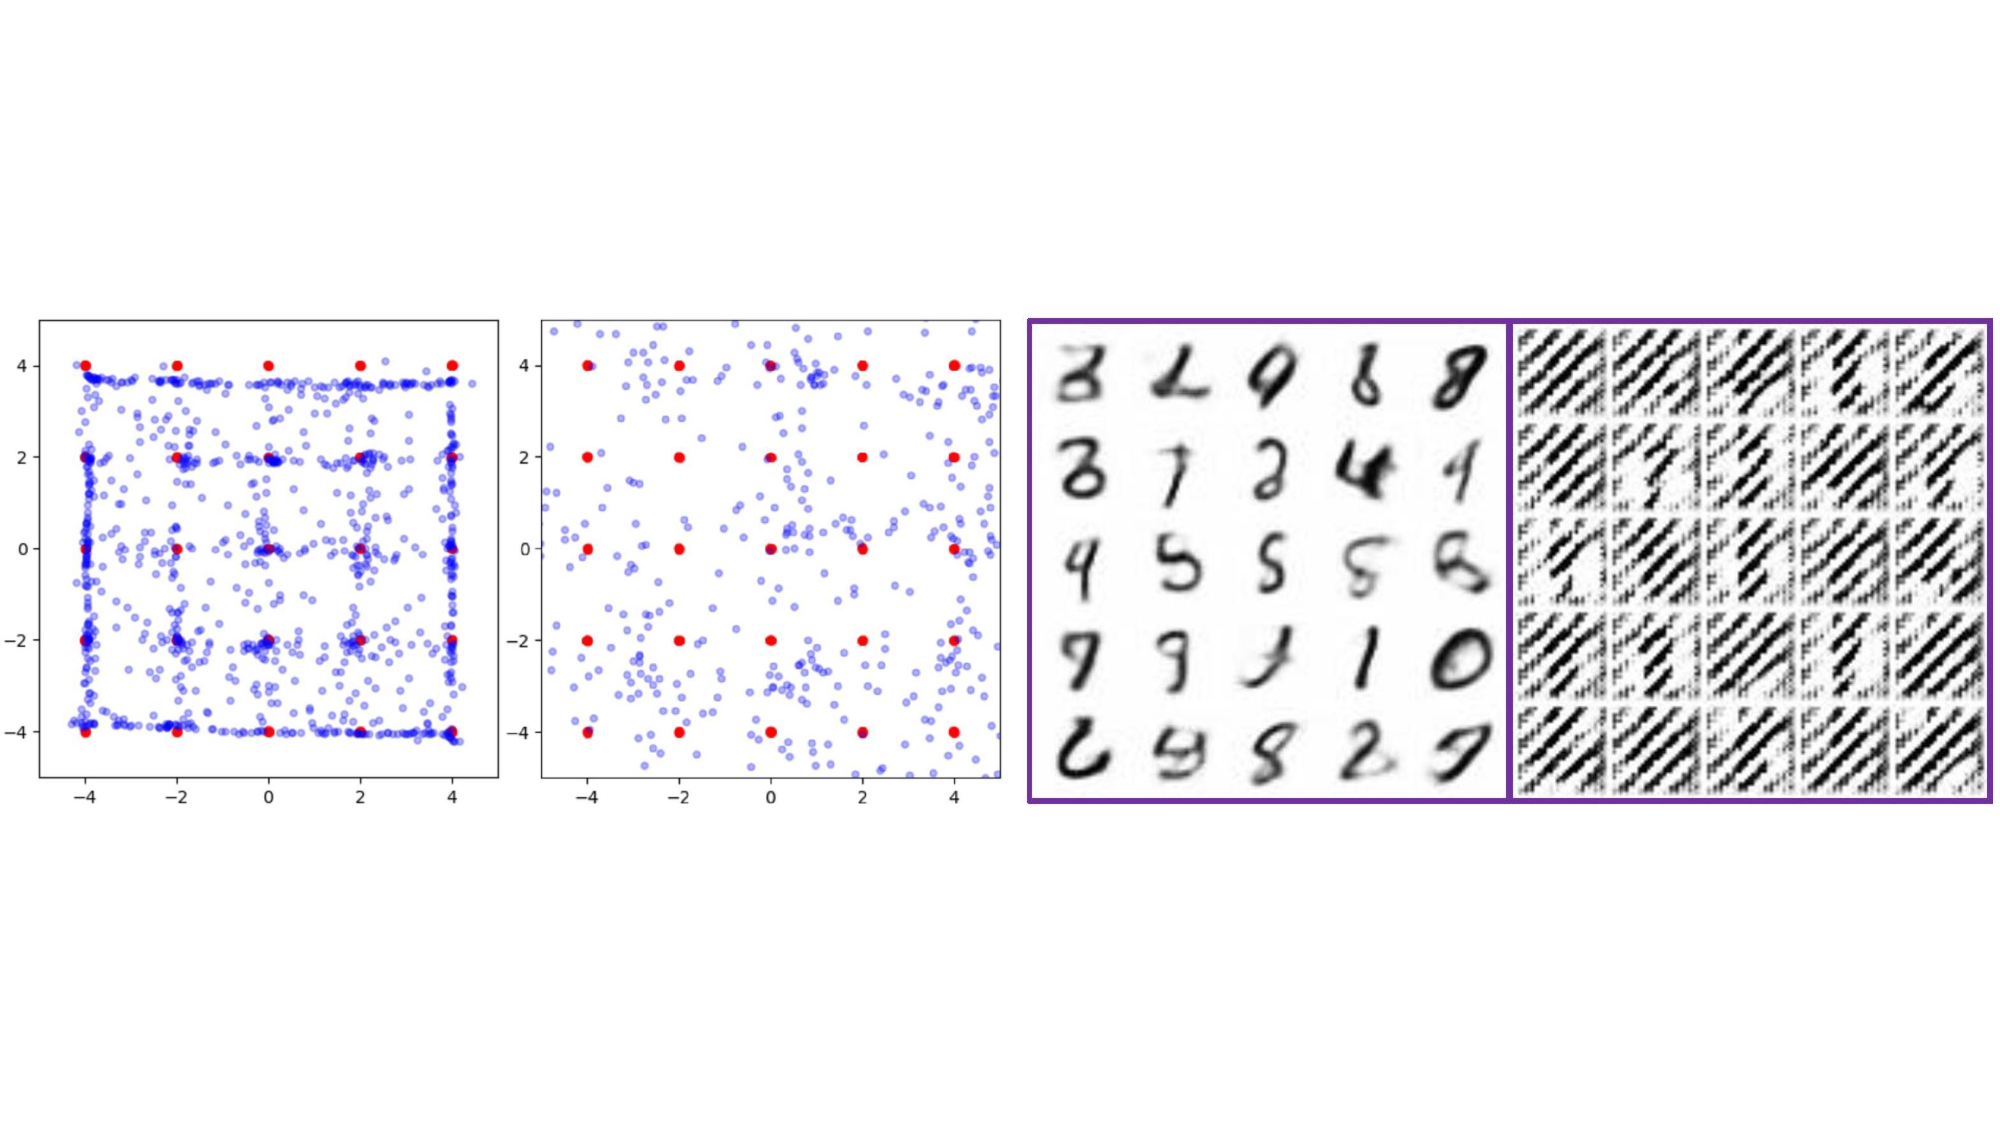
\includegraphics[height=0.23 \columnwidth]{Figures/25GS_MNIST_SN_Forgetting.pdf}
		\caption{
			Demonstration of adversarial learning forgetting the information learned/initialized by ML learning on 25-Gaussians (the first two) and MNIST (the last two). From left to right are the snapshots of ML initialization and $20$ following iterations of adversarial learning, respectively. See
%			Appendix D
			Appendix \ref{sec:ML_AL_explode}
			for details.
		}
		\label{fig:explodes}
\end{figure}


\subsection{Maximum Likelihood Learning (Forward KL)}



A classic method to match a model $p_{\thetav}(\xv)$ to the data distribution $q(\xv)$ is ML learning (or maximum likelihood estimation), namely,
\begin{equation}
\label{eq:ML_loss}
\resizebox{0.98\hsize}{!}{$
\begin{aligned}
    \thetav^{*} & = \argmax_{\thetav} \Ebb_{q(\xv)} [\log p_{\thetav}(\xv)]
%    \\
%    &
    = \argmin_{\thetav} \Dc_{\KL} [q(\xv) \| p_{\thetav}(\xv)],
\end{aligned}
$}
\end{equation}
where $\Dc_{\KL} [q(\xv) \| p_{\thetav}(\xv)] \! = \! \Ebb_{q(\xv)}[\log q(\xv)\! -\! \log p_{\thetav}(\xv)]$ is the forward KL. The gradient wrt $\thetav$ is
\begin{equation}\label{eq:ML_grad}
    {\nabla_{\thetav}} \Dc_{\KL} [q(\xv) \| p_{\thetav}(\xv)]
    = \Ebb_{q(\xv)} [- \nabla_{\thetav} \log p_{\thetav} (x)].
\end{equation}
For more modeling capacity, it is often convenient to define $p_{\thetav}(\xv)$ as the marginal of some parameterized joint distribution $p_{\thetav}(\xv, \zv)$, with latent variable $\zv$. Although $\log p_{\thetav}(\xv)$ is usually intractable, variational inference \cite{jordan1999introduction,kingma2014auto,blei2017variational} seeks to solve the ML learning in \eqref{eq:ML_loss} via maximizing the evidence lower bound (ELBO)
\beq\label{eq:elbo_ML}
\bali
\text{ELBO}(\thetav,\phiv)
= \Ebb_{q(\xv) q_{\phiv}(\zv|\xv)} \big[
\log p_{\thetav}(\xv, \zv) - \log q_{\phiv}(\zv|\xv)
\big],
\eali
\eeq
where $q_{\phiv}(\zv|\xv)$ is the variational approximation with parameters $\phiv$, and the bound is tight when $q_{\phiv}(\zv|\xv) = p_{\thetav}(\zv|\xv)$.
The gradient wrt $\thetav$ becomes
$$
\bali
    {\nabla_{\thetav}}
    & \text{ELBO}(\thetav,\phiv)
    = \Ebb_{q(\xv) q_{\phiv}(\zv|\xv)} [- \nabla_{\thetav} \log p_{\thetav} (\xv, \zv)].
\eali
$$
In practice, $\mathbb{E}_{q(\xv)}[\cdot]$ are approximated as averages over a finite set of observed samples.

\subsection{Adversarial Learning (Reverse KL)}

Recent progress has resulted in many techniques for adversarial training of generative models \cite{goodfellow2014generative,gulrajani2017improved,nowozin2016f,brock2018large}.
The original GAN \cite{goodfellow2014generative} seeks to solve
\begin{equation}\label{eq:GAN_lossd}
\resizebox{0.95\hsize}{!}{$
\begin{aligned}
    \min_{\thetav} \max_{\betav} \Ebb_{q(\xv)} [\log \sigma(f_{\betav}(\xv))]
    + \Ebb_{p_{\thetav} (\xv)} [\log (1-\sigma(f_{\betav}(\xv))) ],
\end{aligned}
$}
\end{equation}
where $\sigma(f_{\betav}(\xv)) \triangleq D_{\betav}(\xv)$ is called the discriminator, $\sigma(a)=1/[1+\exp(-a)]$, and samples are drawn from $p_{\thetav}(\xv)$ by the generative process
\beq\label{eq:p_theta_x_gan}
\bali
\xv \sim \delta(\xv | G_{\thetav}(\zv)), \zv \sim p(\zv),
\eali
\eeq
where $\delta(\xv | \av)$ is the Dirac delta function located at $\av$, $G_{\thetav}(\zv)$ is called the generator, and $p(\zv)$ is an easy-to-sample distribution. It is shown \cite{goodfellow2014generative} that the optimal $\betav^{*}$ for \eqref{eq:GAN_lossd} satisfies
\begin{equation}\label{eq:f_log_ratio}
\begin{aligned}
    f_{\betav^{*}}(\xv) = \log q(\xv) - \log p_{\thetav} (\xv).
\end{aligned}
\end{equation}
Accordingly, \eqref{eq:GAN_lossd} seeks to minimize the Jensen-Shannon (JS) divergence for parameters $\thetav$ \cite{goodfellow2014generative}.


Alternatively, one could also consider a similar GAN objective based on the reverse KL divergence $\Dc_{\KL} [p_{\thetav}(\xv) \| q(\xv)] $ \cite{nowozin2016f,li2019adversarial}, on which we focus in this paper; as discussed in the Introduction, many GANs are closely related \cite{nowozin2016f} and can reach similar performance with the same budget \cite{GoogleCompareGAN}, and therefore a focus on the reverse KL is not deemed particularly limiting. The log-ratio estimate in \eqref{eq:f_log_ratio} is exploited both in the reverse KL and its gradient as
\begin{equation}\label{eq:RKL_loss_grad}
\begin{aligned}
	\bali
    & \Dc_{\KL} [p_{\thetav}(\xv) \| q(\xv)]
    = \Ebb_{p_{\thetav}(\xv)} [-f_{\betav^{*}}(\xv)]
    \\
    & \nabla_{\thetav} \Dc_{\KL} [p_{\thetav}(\xv) \| q(\xv)] =
    \\
    & \qquad \Ebb_{p(\zv)\delta(\xv | G_{\thetav}(\zv))} \big[ -[\nabla_{\thetav} G_{\thetav}(\zv)]
    [\nabla_{\xv} f_{\betav^{*}}(\xv) ] \big].
\eali
\end{aligned}
\end{equation}


\section{Connecting Maximum Likelihood and Adversarial Learning via $\alpha$-Bridge}
\label{sec:Trans}



Maximum likelihood and adversarial learning have many {\em complementary} strengths and weaknesses, motivating development of a method that achieves their principled integration. Toward that end, we propose what we term an $\alpha$-Bridge, designed using the $\alpha$-divergence \cite{cichocki2010families}. The $\alpha$-Bridge smoothly connects the forward and reverse KL divergences, making it possible to transfer advantages from one to the other.


Given model distribution $p_{\thetav}(\xv)$ and the underlying data distribution $q(\xv)$, the $\alpha$-divergence measuring the dissimilarity between these two distributions is defined as
\begin{equation}\label{eq:alpha-div}
    \Dc_{\alpha} [p_{\thetav}(\xv) \| q(\xv)]
    = \frac{1}{\alpha (1 - \alpha)} \Big[
    1 - \int p_{\thetav}(\xv)^{\alpha} q(\xv)^{1-\alpha} d\xv \Big].
\end{equation}
The $\alpha$-divergence has many attractive properties \cite{cichocki2010families}, for example,
($i$) it is unique \cite{amari2009alpha};
($ii$) $\lim_{\alpha \to 0} \Dc_{\alpha} [p_{\thetav} (\xv) \| q(\xv) ] = \Dc_{\KL} [q(\xv) \| p_{\thetav} (\xv) ]$;
($iii$) $\lim_{\alpha \to 1} \Dc_{\alpha} [p_{\thetav}(\xv) \| q(\xv) ] = \Dc_{\KL} [p_{\thetav}(\xv) \| q(\xv) ]$; and
($iv$) the $\alpha$-divergence is a continuous function of $\alpha$.
These properties motivate development of a smooth ``bridge'' via the $\alpha$-divergence, named the $\alpha$-Bridge, to continuously transfer between forward and reverse KL. Before discussing the proposed $\alpha$-Bridge in detail, below we first reveal its key foundation, in the context of this paper: the $\alpha$-divergence has two equivalent expressions for its gradient, which utilize the gradient information either from the forward or reverse KL.

\subsection{Twin Gradients of $\alpha$-Divergence}
\label{sec:Grad}

Given the $\alpha$-divergence defined in \eqref{eq:alpha-div}, with straightforward derivation, we have
\begin{equation}\label{eq:alpha_grad}
\begin{aligned}
    & \nabla_{\thetav} \Dc_{\alpha} [p_{\thetav}(\xv) \| q(\xv)] =
    \\
    &
    \quad \frac{1}{1 - \alpha} \Big[
    - \int p_{\thetav}(\xv)^{\alpha - 1} q(\xv)^{1-\alpha} \nabla_{\thetav} p_{\thetav}(\xv) d\xv \Big].
\end{aligned}
\end{equation}
An interesting fact of \eqref{eq:alpha_grad} is that one can turn it into an expectation-based expression wrt either the data distribution $q(\xv)$ or the model one $p_{\thetav}(\xv)$, resulting in two different expressions for the same gradient
(see
%Appendix A
Appendix \ref{sec:derive_twin_grad}
for details).
By forming expectations wrt $q(\xv)$, we have
\begin{equation}\label{eq:Forward_grad}
\begin{aligned}
    & \nabla_{\thetav} \Dc_{\alpha} [p_{\thetav}(\xv) \| q(\xv)] =
    \\
    &
    \frac{1}{1-\alpha} \Ebb_{q(\xv)} \left[
    -\Big[ \frac{p_{\thetav}(\xv)}{q(\xv)} \Big]^{\alpha}
    \nabla_{\thetav} \log p_{\thetav}(\xv)
    \right]
    \triangleq \nabla_{\thetav} \Dc_{\alpha}^F ,
\end{aligned}
\end{equation}
where $\nabla_{\thetav} \Dc_{\alpha}^F$ is used for brevity. The gradient information from the forward KL in \eqref{eq:ML_grad} serves as a building block for (\ref{eq:Forward_grad}).
However, it is {\em different} from the direct gradient of the forward KL in that $\nabla_{\thetav} \Dc_{\alpha}^F$ has an adaptive ratio-related weight term $\frac{1}{1-\alpha} \big[ \frac{p_{\thetav}(\xv)}{q(\xv)} \big]^{\alpha}$ within the expectation (when $\alpha\rightarrow 0^+$ this term vanishes, leading to the gradient of the forward KL in that limit). For the gradient expression related to $p_{\thetav}(\xv)$ modeled in \eqref{eq:p_theta_x_gan}, we have
\begin{equation}\label{eq:Reverse_grad}
\resizebox{0.95\hsize}{!}{$
\bali
    & \nabla_{\thetav} \Dc_{\alpha} [p_{\thetav}(\xv) \| q(\xv)]
    \triangleq \nabla_{\thetav} \Dc_{\alpha}^R =
    \\
    &
    \Ebb_{p(\zv) \delta(\xv | G_{\thetav}(\zv))} \left[
    [\nabla_{\thetav} G_{\thetav}(\zv)]
    \Big[\frac{q(\xv)}{p_{\thetav}(\xv)} \Big]^{1-\alpha}
    \Big[ \nabla_{\xv} \log \frac{p_{\thetav}(\xv)}{q(\xv)} \Big]
    \right].
\eali
$}
\end{equation}
Similarly we use $\nabla_{\thetav} \Dc_{\alpha}^R$ for brevity. Compared to \eqref{eq:RKL_loss_grad}, $\nabla_{\thetav} \Dc_{\alpha}^R$ utilizes the gradient information from the reverse KL, with another adaptive weighting term $\big[\frac{q(\xv)}{p_{\thetav}(\xv)} \big]^{1-\alpha}$ (which vanishes in the limit $\alpha\rightarrow 1^{-}$, yielding the gradient of the reverse KL in that limit).
For more general model $p_{\thetav}(\xv)$ beyond \eqref{eq:p_theta_x_gan}, the GO gradient \cite{cong2019go} can be utilized to calculate $\nabla_{\thetav} \Dc_{\alpha}^R$.


It is important to note that $\nabla_{\thetav} \Dc_{\alpha}^F$ and $\nabla_{\thetav} \Dc_{\alpha}^R$ are two {\em equivalent} gradient expressions for the same objective $\Dc_{\alpha} [p_{\thetav}(\xv) \| q(\xv)]$, even though they utilize different gradient information (accordingly different MC variance properties as detailed below) from the forward and reverse KL, respectively. Thus, we call them the twin gradients of $\alpha$-divergence. In the limits on $\alpha$, the former is associated with the forward KL and the latter with the reverse KL, but for $\alpha\in (0,1)$ the twin gradients are {\em not} associated with either; this explains why the proposed $\alpha$-Bridge in Sec. \ref{sec:alpha_bridge} is different from a (possibly convex) combination of the forward and reverse KL.

Since $\nabla_{\thetav} \Dc_{\alpha}^F$ and $\nabla_{\thetav} \Dc_{\alpha}^R$ are equivalent expressions for $\nabla_{\thetav} \Dc_{\alpha} [p_{\thetav}(\xv) \| q(\xv)]$, any convex combination of them remains an unbiased gradient estimator, which may be interpreted as exploiting the information from one side to regularize the other side.
We propose to use an $\alpha$-related dynamic combination as
\begin{equation}\label{eq:combine_grad}
\begin{aligned}
\nabla_{\thetav} \Dc_{\alpha} [p_{\thetav}(\xv) \| q(\xv)]
& = (1 - \gamma_{\alpha}) \nabla_{\thetav} \Dc_{\alpha}^F
+ \gamma_{\alpha} \nabla_{\thetav} \Dc_{\alpha}^R,
\end{aligned}
\end{equation}
where $\gamma_{\alpha}$ is specified as a smooth increasing function\footnote{It is consistent with the instinct that, as smoothly transferring from the forward to reverse KL, the used information from the forward/reverse KL should smoothly decrease/increase correspondingly.
%	Appendix E
	Appendix \ref{sec:alpha_w_alpha}
	shows a series of experiments demonstrating several intuitive choices for $\gamma_{\alpha}$. We empirically find that the sigmoid-like function $\gamma_{\alpha} = \frac{\sigma(c\alpha+d) - \sigma(d)}{\sigma(c+d)-\sigma(d)}$ (with hyperparameters $c,d$) works well.
	Accordingly, we use such $\gamma_{\alpha}$ in our experiments and leave as future research how to optimally choose $\gamma_{\alpha}$.
} of $\alpha$ satisfying $\gamma_{0} = 0$, $\gamma_{1}=1$, ensuring equation \eqref{eq:combine_grad} \emph{exactly} recovers the gradient of the forward$/$reverse KL when $\alpha=0 / \alpha=1$.
Such a $\gamma_{\alpha}$ is motivated by the smoothness of the $\alpha$-divergence.
When $\alpha\rightarrow0$ the $\alpha$-divergence smoothly approaches the forward KL with increasingly-similar gradients; intuitively to calculate the gradient $\nabla_{\thetav} \Dc_{\alpha} [p_{\thetav}(\xv) \| q(\xv)]$, one should prefer $\nabla_{\thetav} \Dc_{\alpha}^F$ more as it uses the ML gradient information.
Similarly, $\nabla_{\thetav} \Dc_{\alpha}^R$ is preferred when $\alpha \rightarrow 1$ as it uses the adversarial gradient information and the $\alpha$-divergence now smoothly approaches the reverse KL.
With a simple example, Figure \ref{fig:alpha_grad_var} confirms that intuition by showing that the twin gradients $\nabla_{\thetav} \Dc_{\alpha}^F$ and $\nabla_{\thetav} \Dc_{\alpha}^R$ have complementary variance properties, the former$/$latter having lower MC variance when $\alpha \rightarrow 0 / \alpha \rightarrow 1$.
Figure \ref{fig:alpha_grad_var} also shows that combining the twin gradients as in \eqref{eq:combine_grad} unifies the advantages from both sides and presents a better gradient estimator with lower MC variance for $\alpha \in (0, 1)$.
The twin gradients can be interpreted as control variants to each other.
This is the foundation of our paper, which is further exploited in the following to develop our $\alpha$-Bridge. We are taking the convex combination of two different forms of the {\em same} gradient, which is {\em distinct} from just taking a convex combination of the {\em different} gradients from the forward and reverse KL.

\begin{figure}[tb]
	\centering
	\subcaptionbox{$\mu=3, \sigma=1$ \label{fig:GamAlphaLargeVarMain}}{
%		\includegraphics[height= 2.95 cm]{N_mu_p_compare_3.png}
%		\includegraphics[height= 2.95 cm]{N_std_p_compare_3.png}
		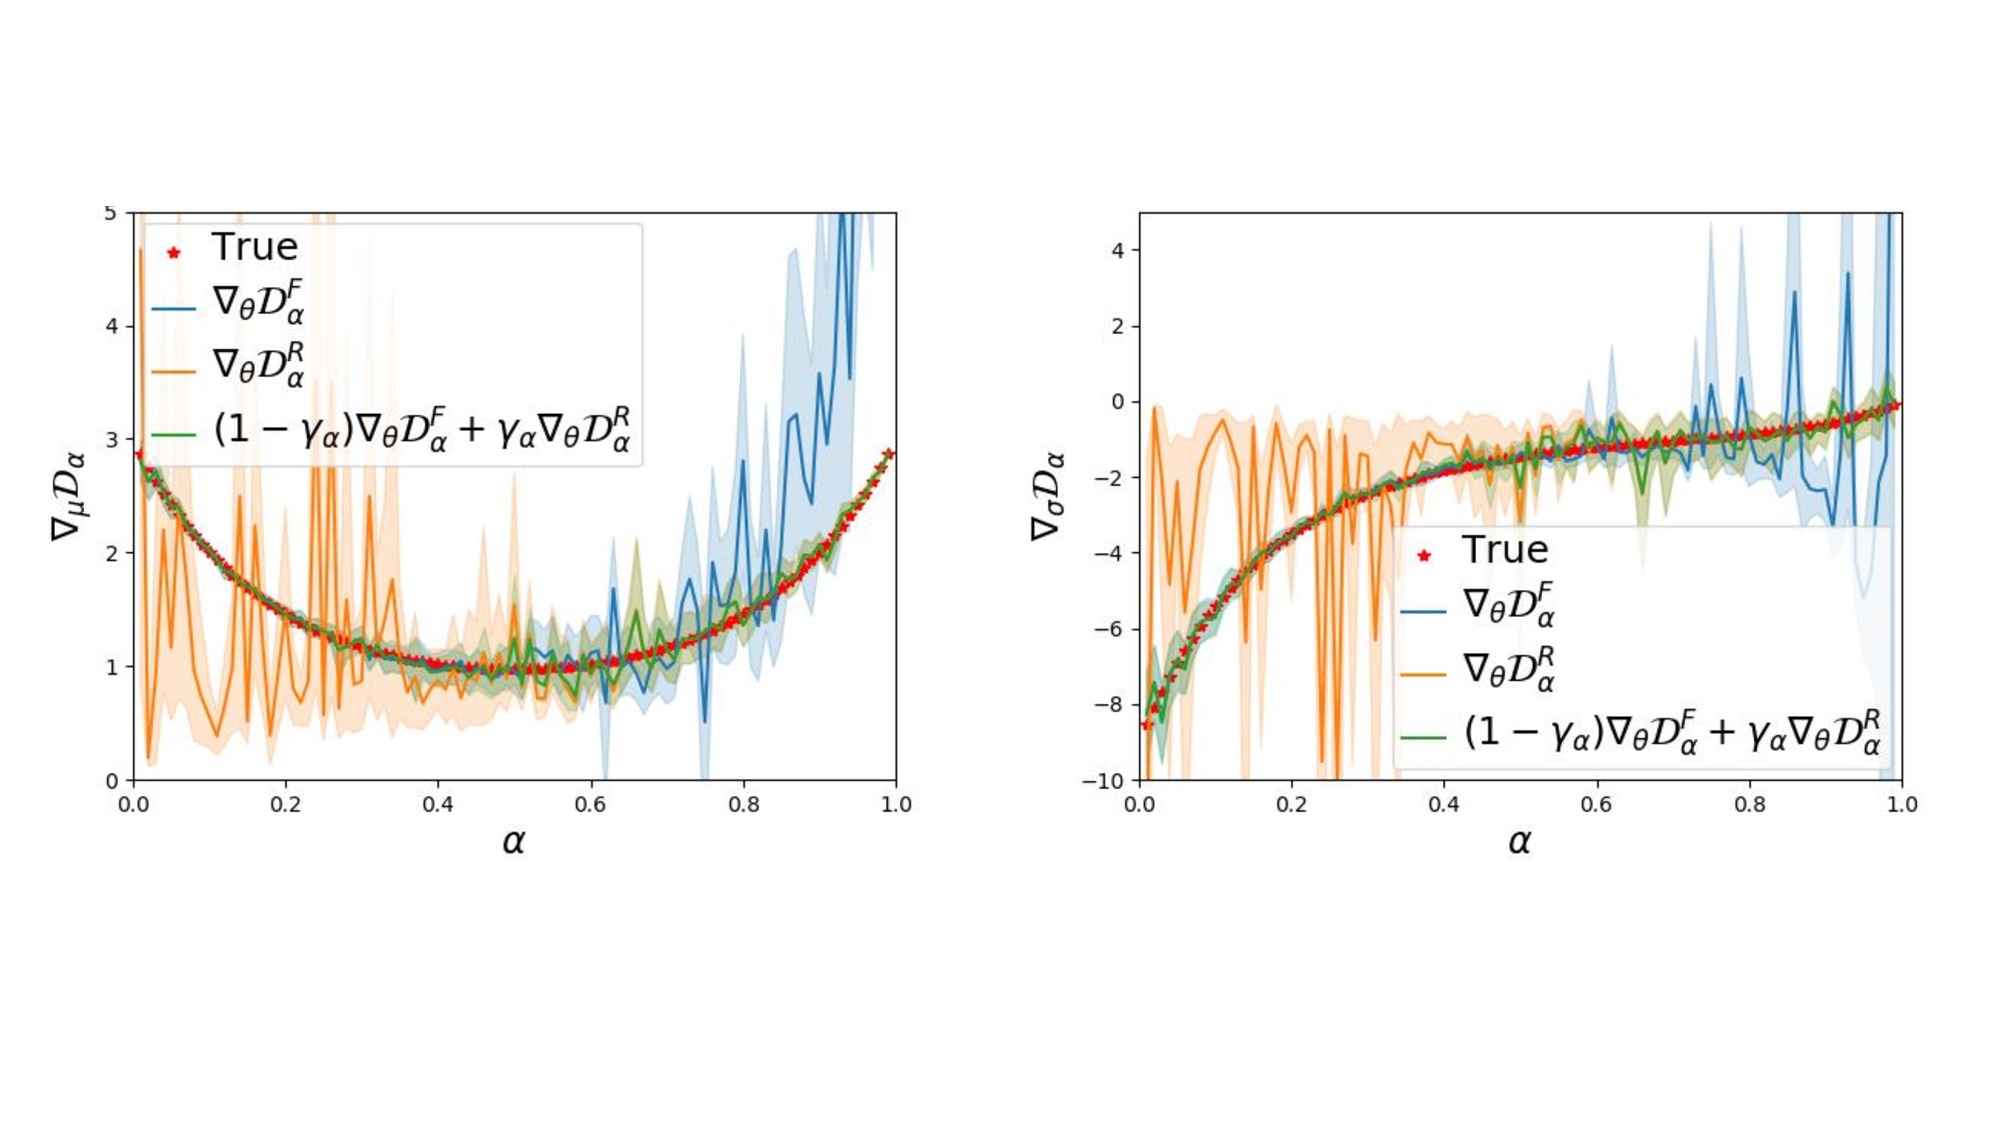
\includegraphics[width= 0.98\columnwidth]{Figures/N_mu_std_p_compare_3.pdf}
	}
	\subcaptionbox{$\mu=1, \sigma=1$ \label{fig:GamELBOMain}}{
%		\includegraphics[height= 2.95 cm]{N_mu_p_compare_1.png}
%		\includegraphics[height= 2.95 cm]{N_std_p_compare_1.png}
		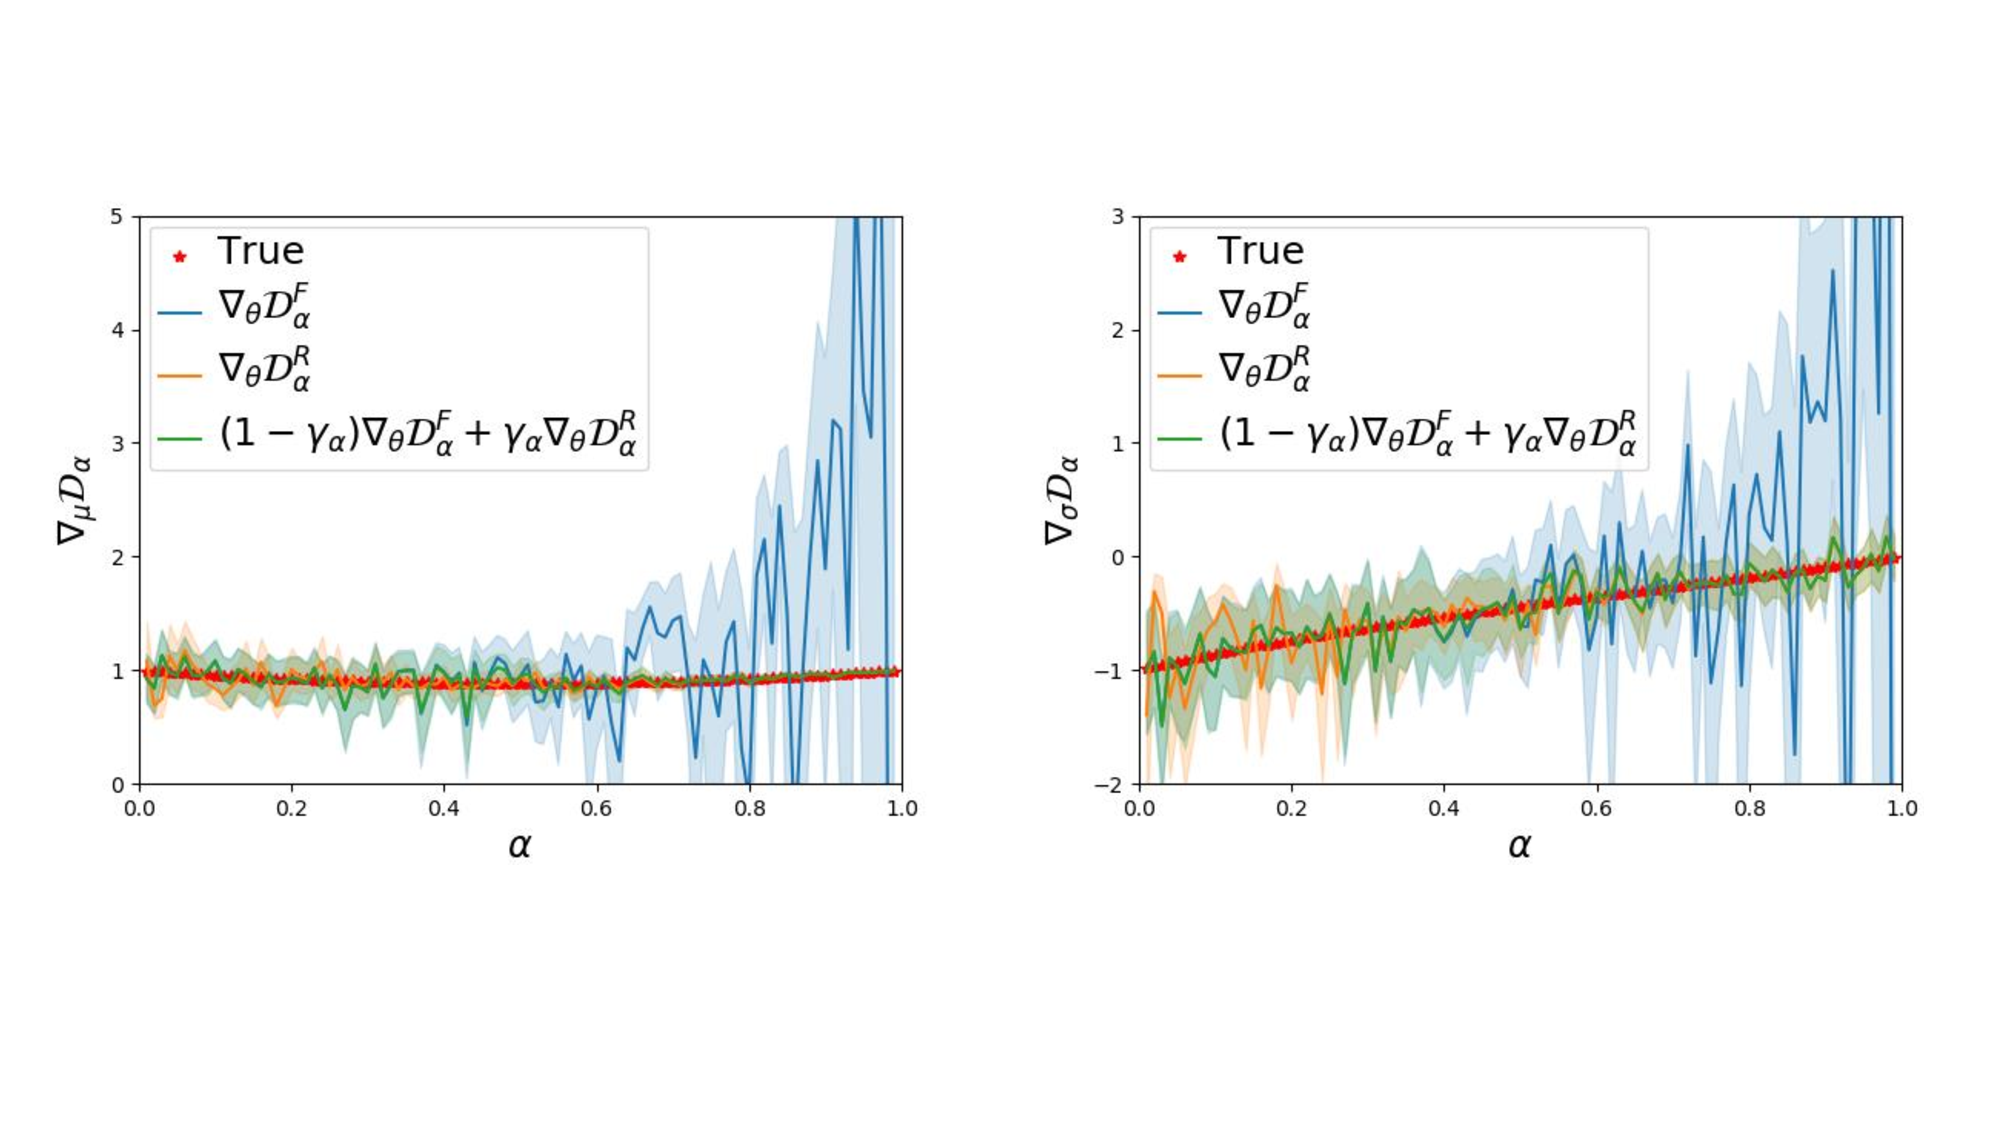
\includegraphics[width= 0.98\columnwidth]{Figures/N_mu_std_p_compare_1.pdf}
	}
	\caption{Illustration of different MC variance properties of different gradient estimators of $\nabla_{\{\mu,\sigma\}}\Dc_{\alpha}[\Nc(x;\mu,\sigma^2)||\Nc(x;0,1)]$ for $\alpha \in (0,1)$.
		$1$ MC sample is used to estimate the gradient. The results are based on $100$ random trials. } \label{fig:alpha_grad_var}
\end{figure}



\begin{algorithm}[tb]
  \caption{$\alpha$-Bridge (from forward to reverse KL)}
  \label{alg:Alpha-divergence}
    \begin{algorithmic}[1]

    \item[\textbf{Input:} Data samples $\xv_i \sim q(\xv)$, an implicit model $p_{\thetav}(\xv)$]

    \item[\textbf{Output:} $\thetav^{*}$ such that $p_{\thetav^{*}}(\xv)$ is closest to the underlying ]
    \item[\qquad\qquad data distribution $q(\xv)$]

      \item[\,\,\, \textit{\textbf{\# Step I: ML learning (forward KL, $\bf \alphav=0$)}}]

      \STATE ML learning for the generator parameter $\thetav$ with the gradient in \eqref{eq:approx_grad_loglike}. Maximizing the ELBO in \eqref{eq:elbo_ML} for training the variational parameters $\phiv$. Pretrain the discriminator parameters $\betav$ with the objective in \eqref{eq:GAN_lossd}.

      \item[\,\,\, \textit{\textbf{\# Step II: Transferring from $\bf \alphav \to 0^{+}$ to $\bf \alphav \to 1^{-}$}}]

      \FOR{$\alpha$ gradually increasing from $0^{+}$ to $1^{-}$}

		\STATE Train $\thetav$ by minimizing the $\alpha$-divergence $\Dc_{\alpha} [p_{\thetav}(\xv) \| q(\xv)]$ with the gradient in \eqref{eq:combine_grad_practical};

		\STATE Train $\phiv$ by maximizing the ELBO in \eqref{eq:elbo_ML};

      	\STATE Train $\betav$ with the objective in \eqref{eq:GAN_lossd};

      \ENDFOR

      \item[\,\,\, \textit{\textbf{\# Step III: Adversarial learning (reverse KL, $\bf \alphav=1$)}}]

      \STATE Refine $\thetav$, $\phiv$, and $\betav$ with the objectives in \eqref{eq:RKL_loss_grad}, \eqref{eq:elbo_ML}, and \eqref{eq:GAN_lossd}, respectively.

    \end{algorithmic}
\end{algorithm}



\subsection{$\alpha$-Bridge via Twin Gradients}
\label{sec:alpha_bridge}




Based on the twin gradients discussed above, we propose a novel $\alpha$-Bridge to dynamically transfer between forward KL (ML learning) and reverse KL (adversarial learning), so as to unify the advantages from both ends\footnote{See
%	Appendix H
	Appendix \ref{sec:other_poten_gener}
	for detailed discussions on other potential generalizations of $\alpha$-Bridge.}.
In this paper, we are motivated by applications associated with GAN, with a goal of generating realistic samples from our model. Accordingly, we set our $\alpha$-Bridge to transfer from the forward KL to the reverse KL, in order to gradually transfer the advantages (see Table \ref{tab:forward_reverse_KL_pro_con}) of ML learning to adversarial learning.
Specifically, we propose to train $p_{\thetav}(\xv)$ via the $\alpha$-Bridge with the following three successive steps.

In Step $I$, we adopt ML learning (forward KL, $\alpha=0$) for efficient initialization thanks to its mode-covering and stable-training properties. One can skip this step if pretrained models from ML learning are available.
From the perspective of practical implementation, one often need to approximately calculate the gradient in \eqref{eq:ML_grad}, as $p_{\thetav}(\xv)$ may be intractable for example for the implicit model in \eqref{eq:p_theta_x_gan}.
For this issue, we first add small Gaussian noise\footnote{We need not to add the noise if $p_{\thetav}(\xv)$ is modeled as \eqref{eq:tilde_p_theta_x_joint} in the first place, for example to take into consideration the widely-existing observation noise of data. See
%Appendix B
Appendix \ref{sec:app_semi_implicit}
for details. }
on top of the generative process of $p_{\thetav}(\xv)$ to form a semi-implicit surrogate model \cite{yin2018semi}
$
\tilde p_{\thetav}(\xv): \xv \sim \Nc(\xv | \xv', \sigma^2 \Imat), \xv' \sim p_{\thetav}(\xv'),
$
for which we have $\nabla_{\thetav} \log p_{\thetav}(\xv) = \lim_{\sigma^2 \to 0} \nabla_{\thetav} \log \tilde p_{\thetav}(\xv)$.
Observing that $\tilde p_{\thetav}(\xv)$ is equivalent to
\beq\label{eq:tilde_p_theta_x_joint}
\tilde p_{\thetav}(\xv): \xv \sim \Nc(\xv | G_{\thetav}(\zv), \sigma^2 \Imat), \zv \sim p(\zv),
\eeq
which has computable joint distribution $\tilde p_{\thetav}(\xv , \zv)$,
we then use the ELBO technique to get
\beq\label{eq:approx_grad_loglike}
\bali
\nabla_{\thetav} \log p_{\thetav}(\xv)
& \approx \nabla_{\thetav} \log \tilde p_{\thetav}(\xv)
\\ &
= \Ebb_{q(\xv) q_{\phiv^{*}}(\zv|\xv)} \big[
\nabla_{\thetav} \log \tilde p_{\thetav}(\xv, \zv)
\big],
\eali
\eeq
with an additional variational inference arm.



In the middle Step $I\!I$, we continue the training of $p_{\thetav}(\xv)$ by gradually changing $\alpha$ from $0^{+}$ to $1^{-}$, so as to transfer what's learned during Step $I$ to the next Step $I\!I\!I$ (reverse-KL-based adversarial learning, $\alpha=1$).
The gradient of the $\alpha$-divergence in \eqref{eq:combine_grad} is used during training. The same techniques discussed above is adopted to calculate the $\nabla_{\thetav} \log p_{\thetav}(\xv)$ term within $\nabla_{\thetav} \Dc_{\alpha}^F$ in \eqref{eq:Forward_grad}.
To calculate the density-ratio-related terms in both $\nabla_{\thetav} \Dc_{\alpha}^F$ and $\nabla_{\thetav} \Dc_{\alpha}^R$ (see \eqref{eq:Forward_grad} and \eqref{eq:Reverse_grad}), we follow the common practice in the GAN literature to solve \eqref{eq:GAN_lossd} for $f_{\betav^{*}}(\xv)$ in \eqref{eq:f_log_ratio}.
Accordingly, we have $\frac{p_{\thetav}(\xv)}{q(\xv)} = e^{-f_{\betav^{*}}(\xv)}$, $\nabla_{\xv} \log \frac{p_{\thetav}(\xv)}{q(\xv)} = -\nabla_{\xv} f_{\betav^{*}}(\xv)$, and
\begin{equation}\label{eq:combine_grad_practical}
\resizebox{1\hsize}{!}{$
	\begin{aligned}
	& \nabla_{\thetav} \Dc_{\alpha} [p_{\thetav}(\xv) \| q(\xv)] \approx
	\\&  \frac{1 - \gamma_{\alpha}}{1 - \alpha} \Ebb_{q(\xv) q_{\phiv^{*}}(\zv|\xv)} \big[ -
	e^{- \alpha f_{\betav^{*}}(\xv)}
	\nabla_{\thetav} \log \tilde p_{\thetav}(\xv, \zv)
	\big] +
	\\
	& \gamma_{\alpha} \Ebb_{p(\zv) \delta(\xv | G_{\thetav}(\zv))} \Big[ -
	[\nabla_{\thetav} G_{\thetav}(\zv)]
	e^{(1 - \alpha) f_{\betav^{*}}(\xv)}
	\big[ \nabla_{\xv} f_{\betav^{*}}(\xv) \big]
	\Big],
	\end{aligned}
	$}
\end{equation}
which combines the gradient information from ML and adversarial learning with automatic weights related to both $\alpha$ and the GAN discriminator.


Finally in Step $I\!I\!I$, we use the zero-forcing reverse-KL-based adversarial learning ($\alpha=1$) to continually refine the generator parameters $\thetav$ and the discriminator parameters $\phiv$ using \eqref{eq:RKL_loss_grad} and \eqref{eq:GAN_lossd}, respectively. The corresponding training process is summarized in Algorithm \ref{alg:Alpha-divergence}.





\subsection{Connections to Prior GAN-Learning Regularization} \label{sec:insight}



Considering the aforementioned twin gradients and the $\alpha$-Bridge, we next present an interpretation of the gradient in \eqref{eq:combine_grad_practical}, with which we reveal two generalizations that are highly related to CycleGAN \cite{zhu2017unpaired} and ALICE \cite{li2017alice}. Details are given in
%Appendix C.
Appendix \ref{sec:Two_connections_cycle}.
With $\mathbox{\xv}$ denoting the stop-gradient operator\footnote{{tf.stop\_gradient}$/${torch.no\_grad} in TensorFlow/PyTorch.}, the gradient in \eqref{eq:combine_grad_practical} can be reformulated as
\begin{equation}\label{eq:cycle_reverseKL}
\resizebox{1\hsize}{!}{$
\begin{aligned}
    & \nabla_{\thetav} \Dc_{\alpha} [p_{\thetav}(\xv) \| q(\xv)] \approx
    \\
    &
    \nabla_{\thetav} \left[
    \bali
        & \frac{1 - \gamma_{\alpha}}{1 - \alpha}
        \Ebb_{q(\xv) q_{\phiv^{*}}(\zv|\xv)} \Big[
        \frac{e^{- \alpha f_{\betav^{*}}(\xv)}}{ 2\sigma^2}
        \| \xv - G_{\thetav}(\zv) \|_2^2
        \Big]
        \\
        & + \gamma_{\alpha} \Ebb_{p_{\thetav}(\xv)} \big[
        -e^{(1 - \alpha) f_{\betav^{*}}(\mathbox{\xv})}
        f_{\betav^{*}}(\xv)
        \big]
    \eali
    \right],
\end{aligned}
$}
\end{equation}
where the first term can be interpreted as weighted half cycle-consistency \cite{li2017alice,zhu2017unpaired,kim2017learning},
and the second one is related to the reverse-KL-based adversarial learning.
Based on the interpretation in \eqref{eq:cycle_reverseKL}, one can readily verify (see
%Appendix C)
Appendix \ref{sec:Two_connections_cycle})
that by generalizing the $\alpha$-Bridge derivations as in \eqref{eq:cycle_reverseKL} to consider both marginals
$$
\resizebox{0.95\hsize}{!}{$
\bali
& \Dc_{\alpha} [p_{\thetav}(\xv) \| q(\xv)] + \Dc_{\alpha} [q_{\phiv}(\zv) \| p(\zv)]
\\
&
\overset{\nabla}{\approx}
\left[
\bali
& \frac{1 - \gamma_{\alpha}}{1 - \alpha} \Ebb_{q(\xv) q_{\mathbox{\phiv}}(\zv|\xv)} \Big[
\frac{e^{- \alpha f_{\betav^{*}}(\xv)}}{2\sigma^2}
\| \xv - G_{\thetav}(\zv) \|_2^2
\Big]
\\
& + \frac{1 - \gamma_{\alpha}}{1 - \alpha} \Ebb_{p(\zv) p_{\mathbox{\thetav}}(\xv|\zv)} \Big[
\frac{e^{- \alpha g_{\gammav^{*}}(\zv)}}{2\sigma^2}
\| \zv - E_{\phiv}(\xv) \|_2^2
\Big]
\\
& + \gamma_{\alpha} \Ebb_{p_{\thetav}(\xv)} \Big[
-e^{(1 - \alpha) f_{\betav^{*}}(\mathbox{\xv})}
f_{\betav^{*}}(\xv)
\Big]
\\
& + \gamma_{\alpha} \Ebb_{q_{\phiv}(\zv)} \Big[
-e^{(1 - \alpha) g_{\gamma^{*}}(\mathbox{\zv})}
g_{\gammav^{*}}(\zv)
\Big]
\eali
\right],
\eali
$}
$$
where $\overset{\nabla}{\approx}$ means both sides have approximately equal gradients mimicking \eqref{eq:cycle_reverseKL}, and $g_{\gammav^{*}}(\zv)= \log p(\zv) - \log q_{\phiv} (\zv)$ corresponds to the optimal discriminator in the $\zv$ space.
Similarly, by considering both joint distributions
$$
\resizebox{0.95\hsize}{!}{$
\bali
& \Dc_{\alpha} [p_{\thetav}(\xv, \zv) \| q_{\mathbox{\phiv}}(\xv,\zv)]] + \Dc_{\alpha} [q_{\phiv}(\xv,\zv) \| p_{\mathbox{\thetav}}(\xv, \zv)]]
\\
&
\overset{\nabla}{\approx}
\left[
\bali
& \frac{1 - \gamma_{\alpha}}{1 - \alpha} \Ebb_{q_{\mathbox{\phiv}}(\xv,\zv)} \big[ -
e^{- \alpha h_{\etav^{*}}(\xv, \zv)}
\log p_{\thetav}(\xv| \zv)
\big]
\\
& + \frac{1 - \gamma_{\alpha}}{1 - \alpha} \Ebb_{p_{\mathbox{\thetav}}(\xv, \zv)} \Big[
-e^{ \alpha h_{\etav^{*}}(\xv, \zv)}
\log q_{\phiv}(\zv | \xv) \Big]
\\
& + \gamma_{\alpha} \Ebb_{p_{\thetav}(\xv, \zv)} \big[-
e^{(1 - \alpha) h_{\etav^{*}}(\mathbox{\xv}, \zv)}
h_{\etav^{*}}(\xv, \zv)
\big]
\\
& + \gamma_{\alpha} \Ebb_{q_{\phiv}(\xv,\zv)} \big[
e^{-(1 - \alpha) h_{\etav^{*}}(\xv, \mathbox{\zv})}
h_{\etav^{*}}(\xv, \zv)
\big]
\eali
\right],
\eali
$}
$$
one can generalize the $\alpha$-Bridge to a model very much resembling ALICE \cite{li2017alice}. We believe that the connections revealed above, and the techniques developed earlier, may be helpful for constituting a foundation that unifies ML learning, adversarial learning, and intuitive (regularization) properties like cycle-consistency.



\section{Related Work}


Motivated by the complementary properties of ML and adversarial learning, many methods have been considered for combining these two popular research fields, to unify their advantages.
A direct combination of the VAE with GAN objectives was considered in \cite{larsen2015autoencoding}, only to ``observe the devil in the details'' during model development and training. Accordingly gradients were heuristically controlled in back-propagation.
It is also stated in \cite{mathieu2016disentangling} that naively combining
those two objectives unstabilizes the system and does not lead to perceptually better generation, which is consistent with the empirical results from \cite{zhang2019training}.
The principle combination of ML and adversarial learning deserves a thorough exploration.
Instead of directly combining their objectives, the $\alpha$-Bridge dynamically transfers (information) between both sides to bypass the unstable problem.
Many other works combining ML and adversarial learning were motivated differently. On the one hand, with the target of ML learning unchanged, \cite{makhzani2015adversarial,mescheder2017adversarial} exploited GAN techniques to better handle the KL term between the prior and posterior of the latent variables, within the ELBO. On the other hand, keeping the target of adversarial learning, a variational auto-encoder/autoencoder was used as a building block within GAN discriminators, mainly for stabilizing training
\cite{berthelot2017began,ulyanov2018takes}.
A symmetric KL divergence was exploited to build objectives \cite{pu2017adversarial,chen2018symmetric}. Since those methods employed discriminators to estimate/replace the ratios within both the forward and reverse KL, the likelihood (gradient) information from forward KL was ignored.
By comparison, the $\alpha$-Bridge has the advantage of benefiting from the gradient information from ML learning.
Although combining ML and adversarial learning is enticing, no previous work has achieved this in a principled manner.
The proposed $\alpha$-Bridge seeks to fill this gap.



\begin{figure}[tb]
	\centering
	%		\includegraphics[width=0.85\columnwidth]{25Gs_GenProcess_GP.pdf}
	%		\includegraphics[width=0.85\columnwidth]{25Gs_GenProcess_SN.pdf}
	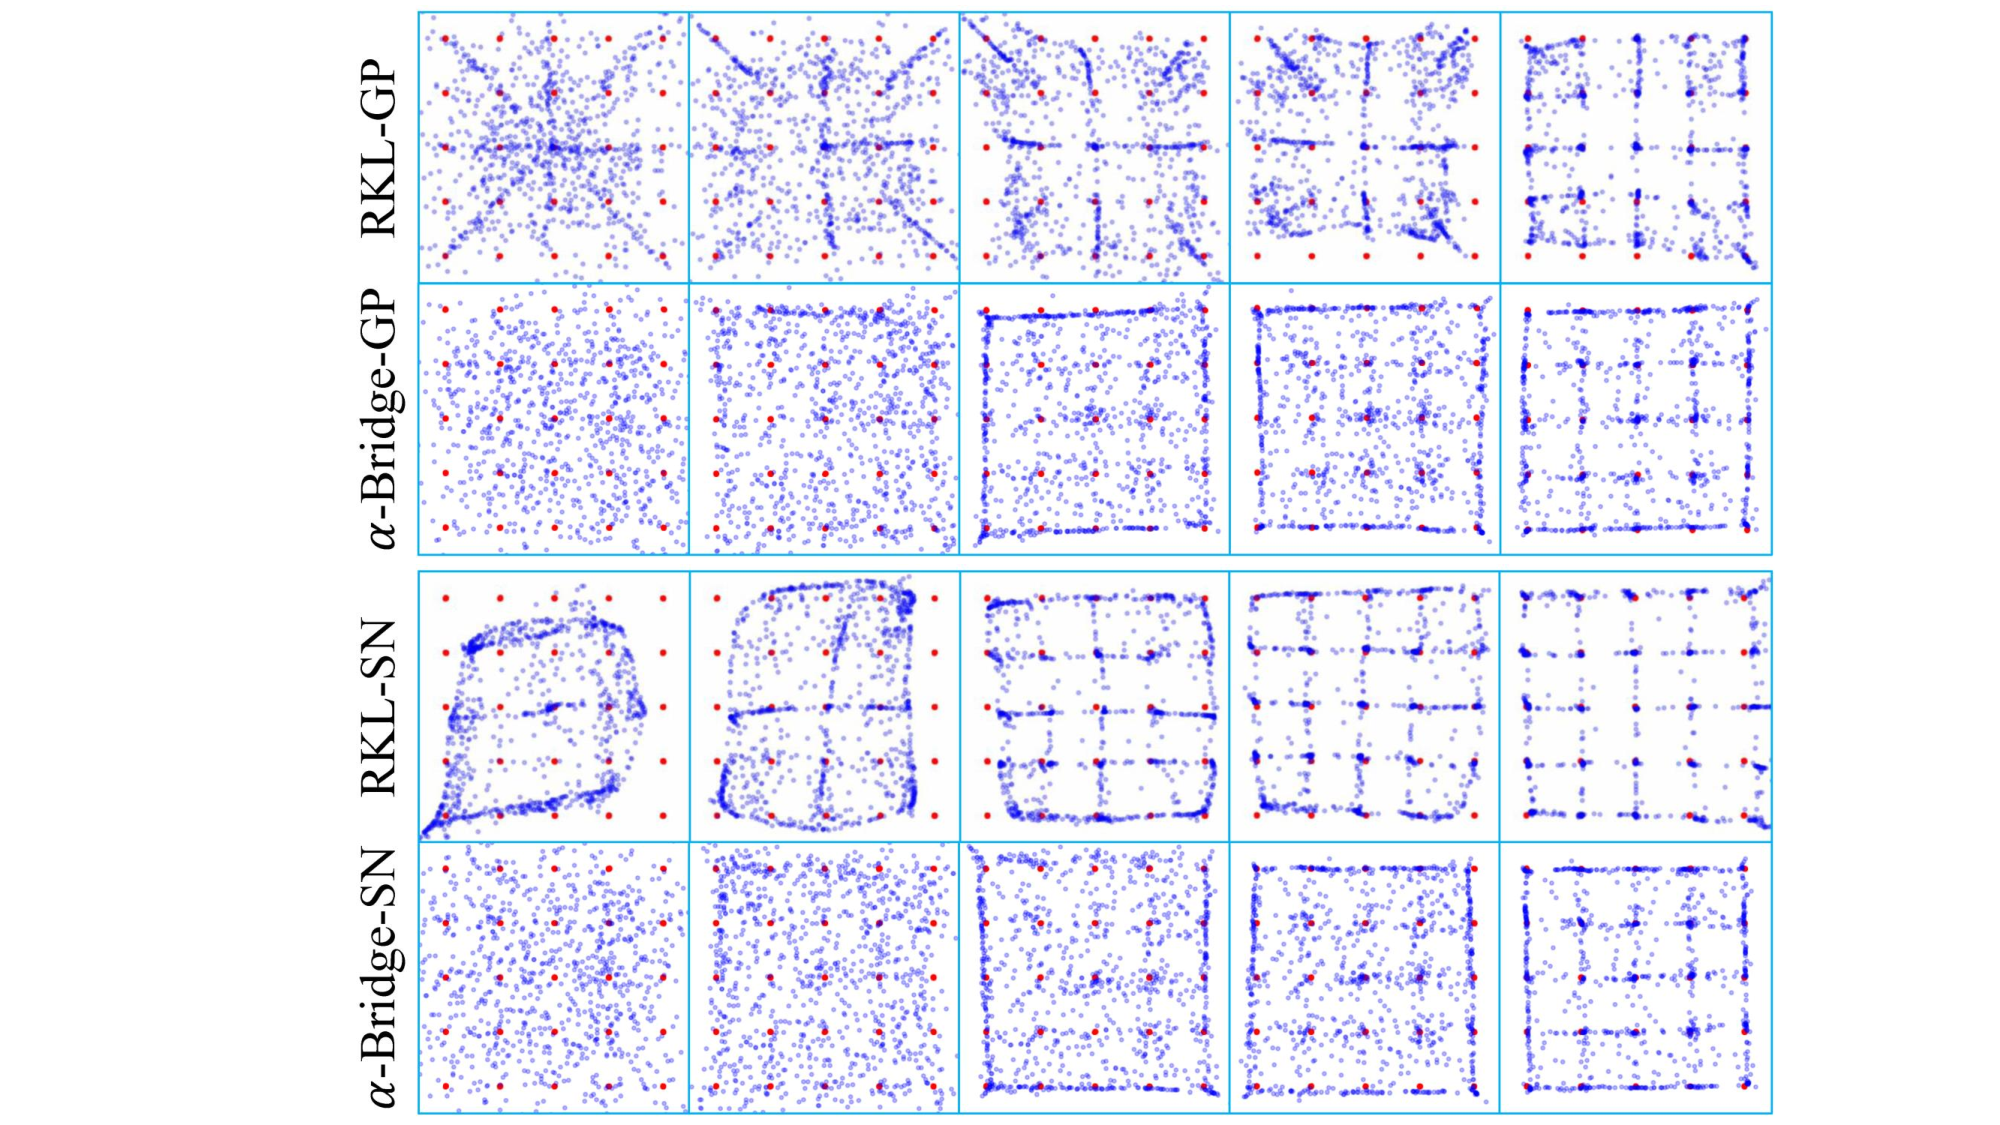
\includegraphics[width=0.85\columnwidth]{Figures/25Gs_GenProcess_GP_SN.pdf}
	\caption{Demonstration on the dynamic evolution of the generated samples (blue) from the compared methods during training. Columns correspond to 1K, 2K, 4K, 6K, and 10K iterations. Real data samples are shown in red.
	}
	\label{fig:Sample_25G}
\end{figure}



\section{Experiments}
\label{sec:Experim}



\begin{figure}[tb]
	\centering
	\subcaptionbox{$\beta_1=0.1$ \label{fig:25Gs_4IS_0_1}}[.48\linewidth]{
		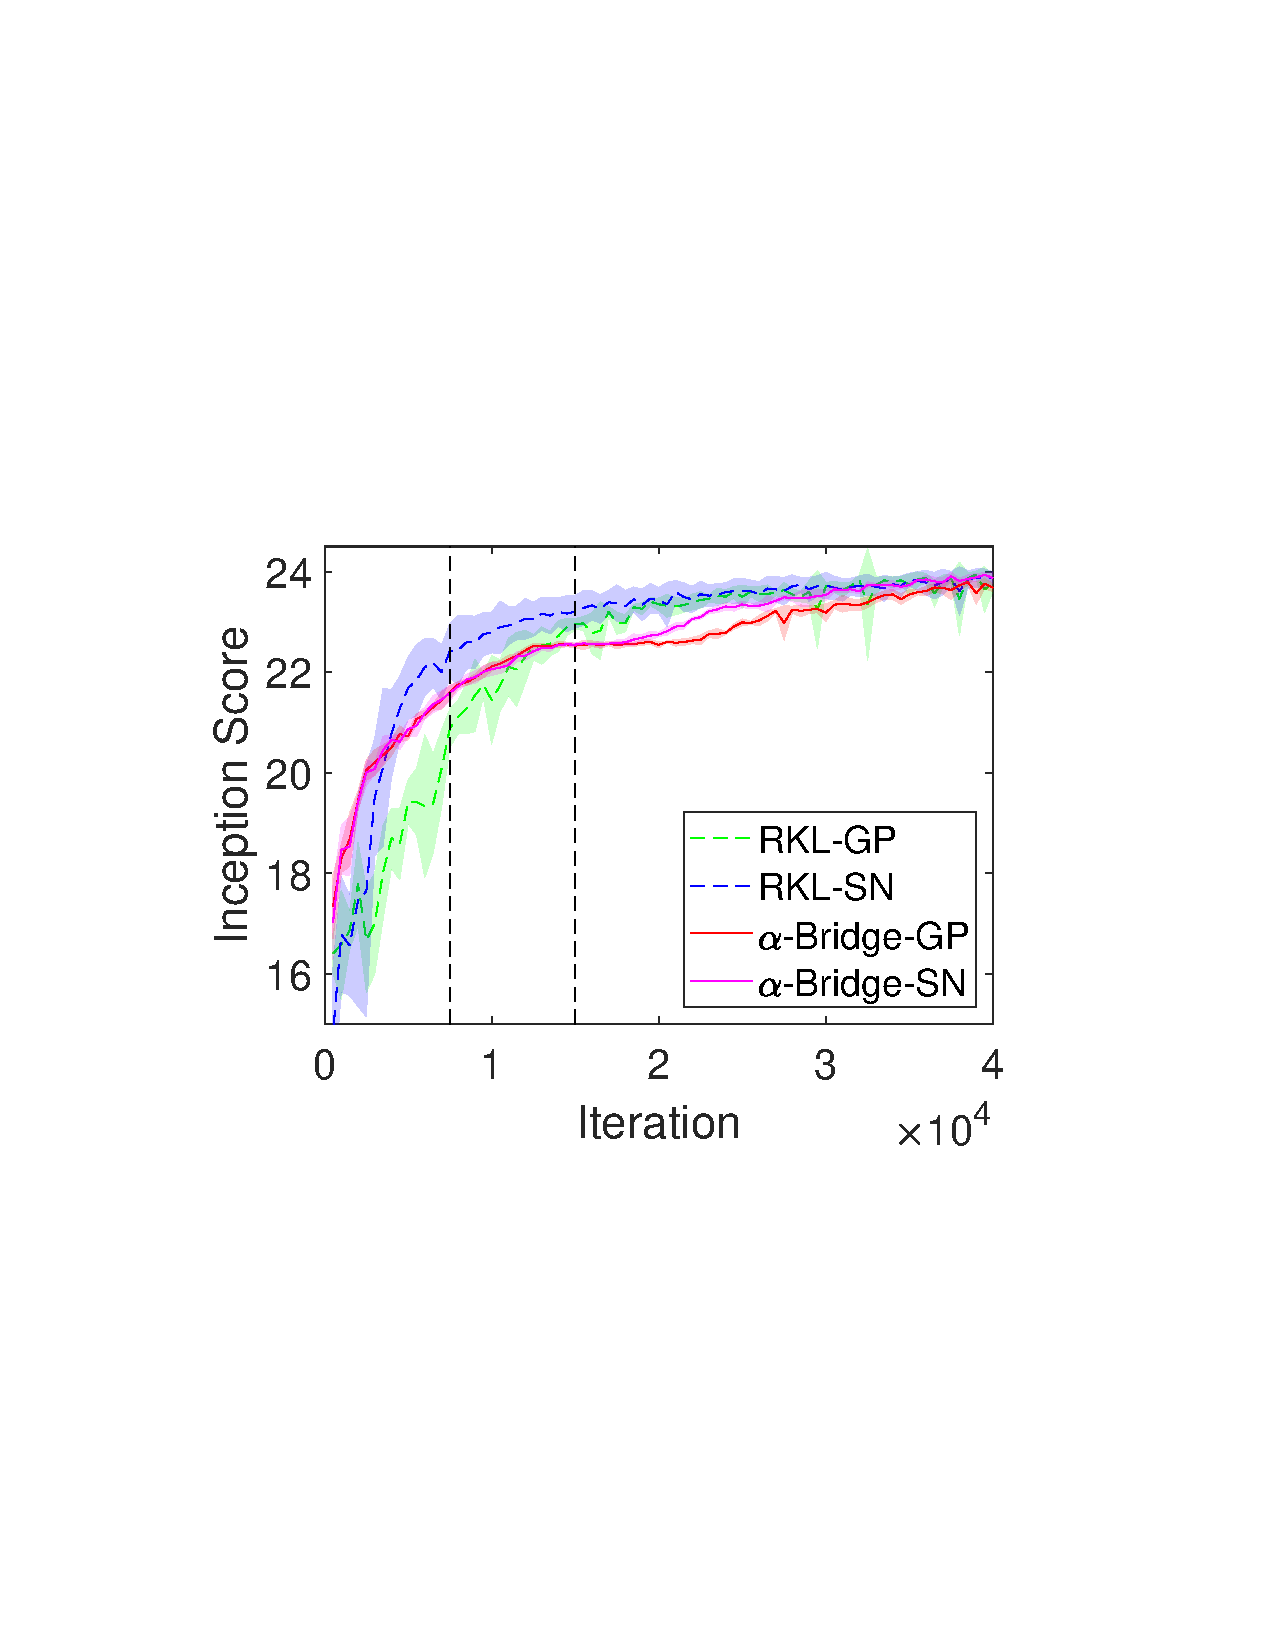
\includegraphics[height=0.33 \columnwidth]{Figures/0-5KL_25Gs_4comErr_IS_2e4_0_1.pdf}
	}
	\subcaptionbox{$\beta_1=0.1$ \label{fig:25Gs_4LL_0_1}}[.48\linewidth]{
		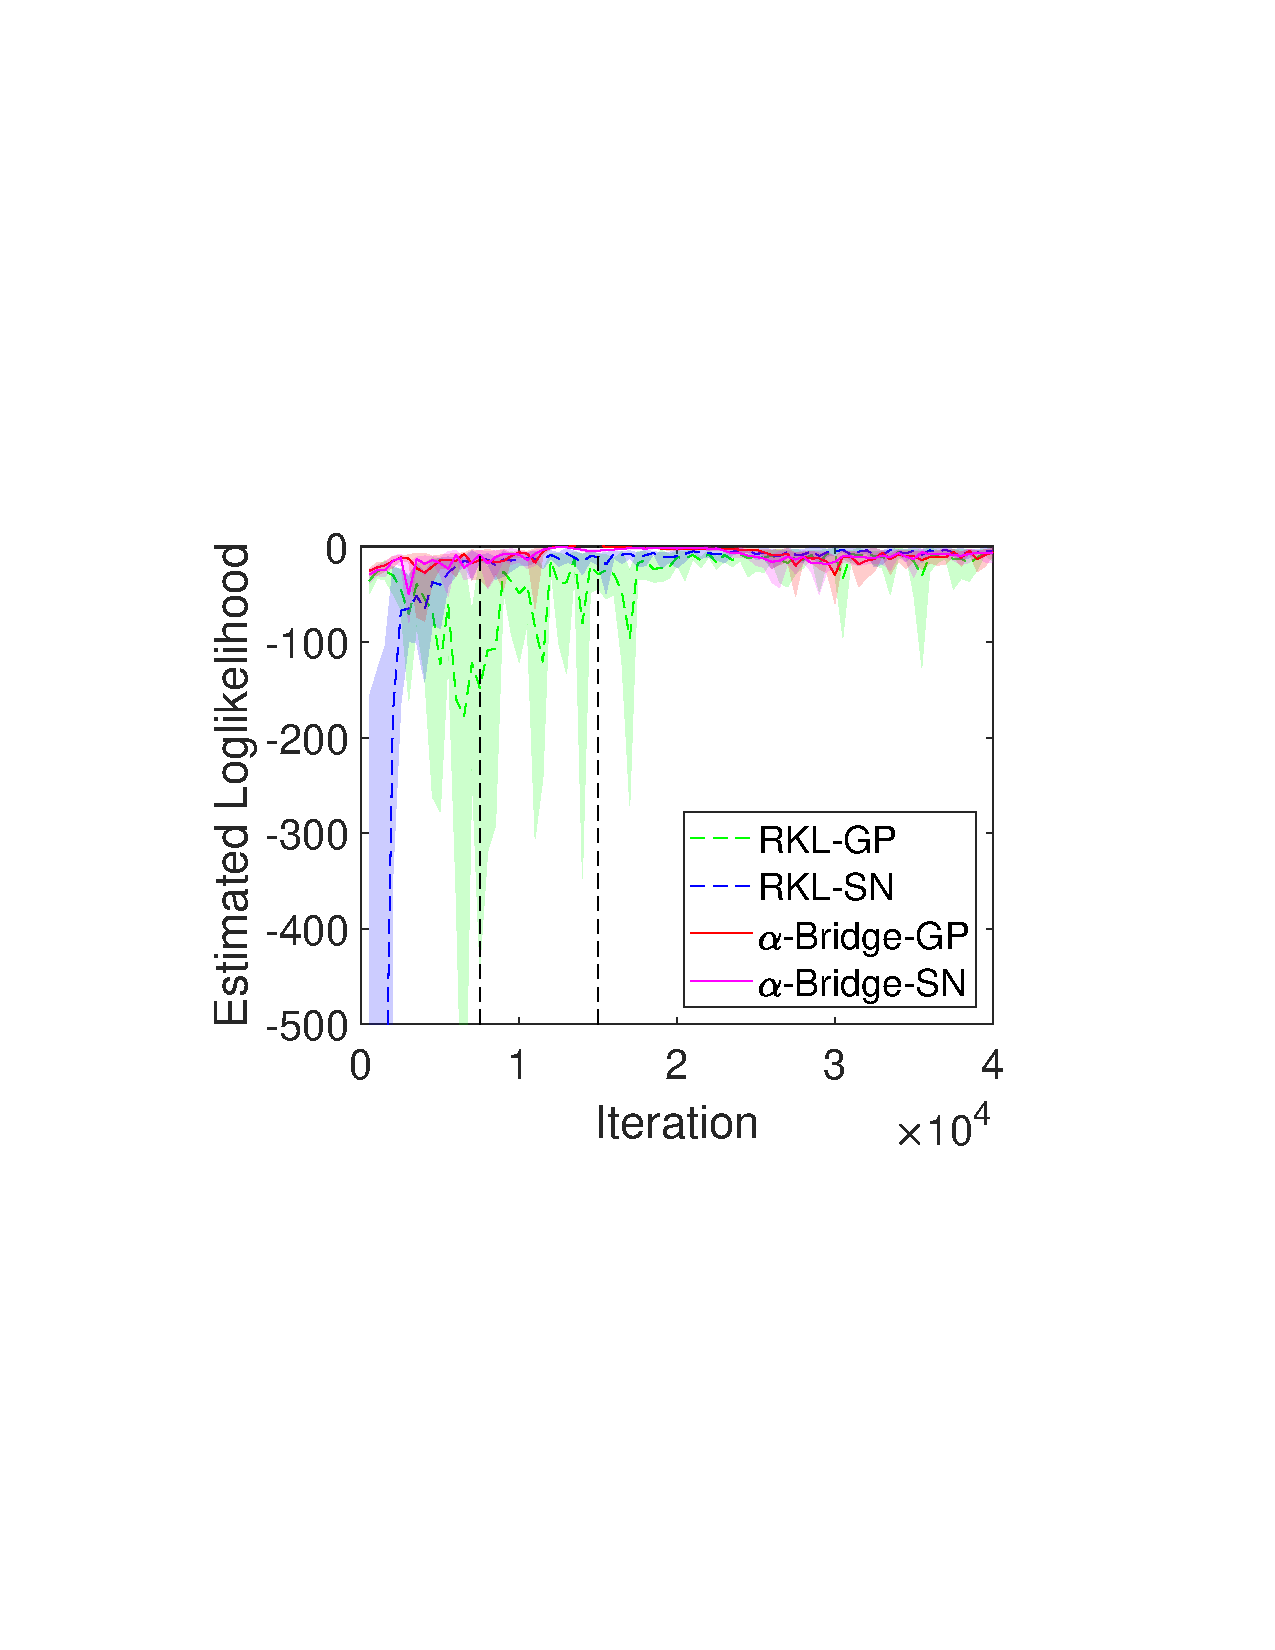
\includegraphics[height=0.33 \columnwidth]{Figures/0-5KL_25Gs_4comErr_loglikehood_2e4_0_1.pdf}
	}
	\subcaptionbox{$\beta_1=0.5$ \label{fig:25Gs_4IS_0_5}}[.48\linewidth]{
		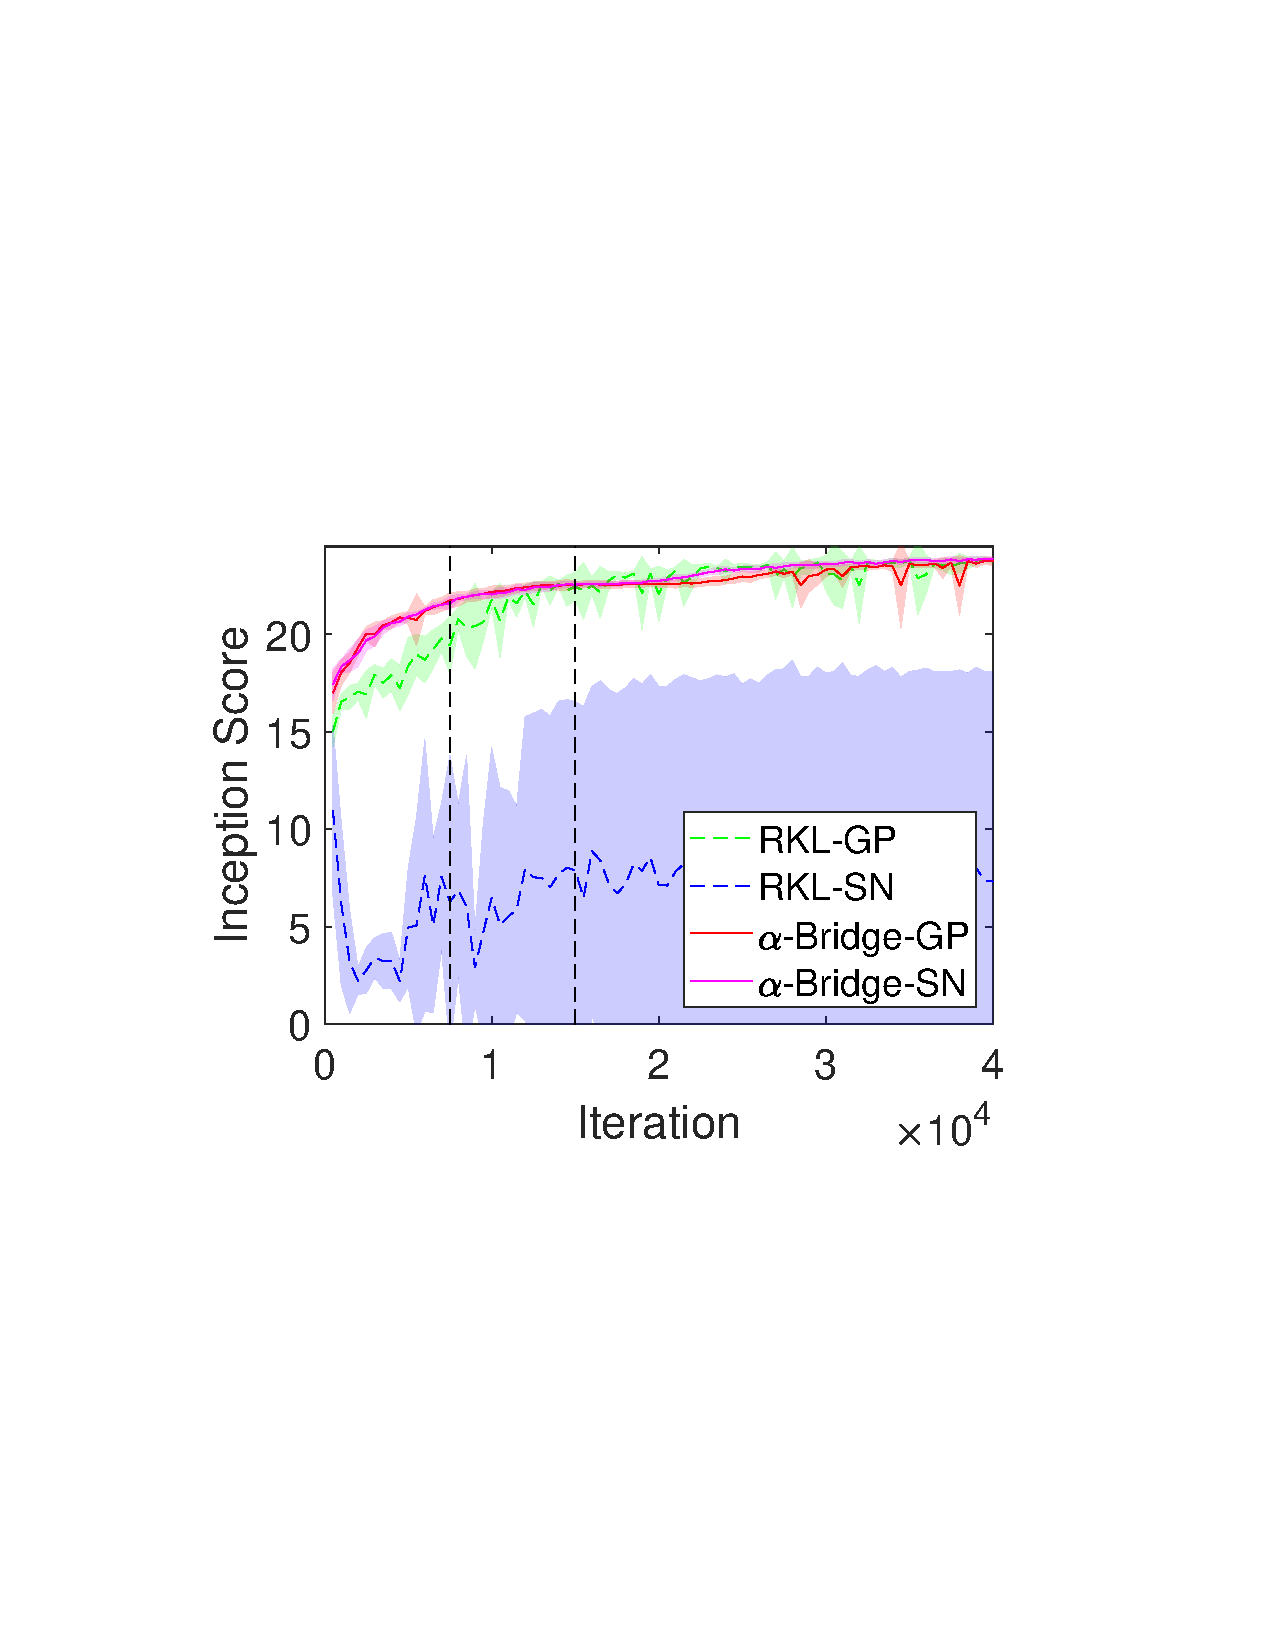
\includegraphics[height=0.33 \columnwidth]{Figures/0-5KL_25Gs_4comErr_IS_2e4_0_5.pdf}
	}
	\subcaptionbox{$\beta_1=0.5$ \label{fig:25Gs_4LL_0_5}}[.48\linewidth]{
		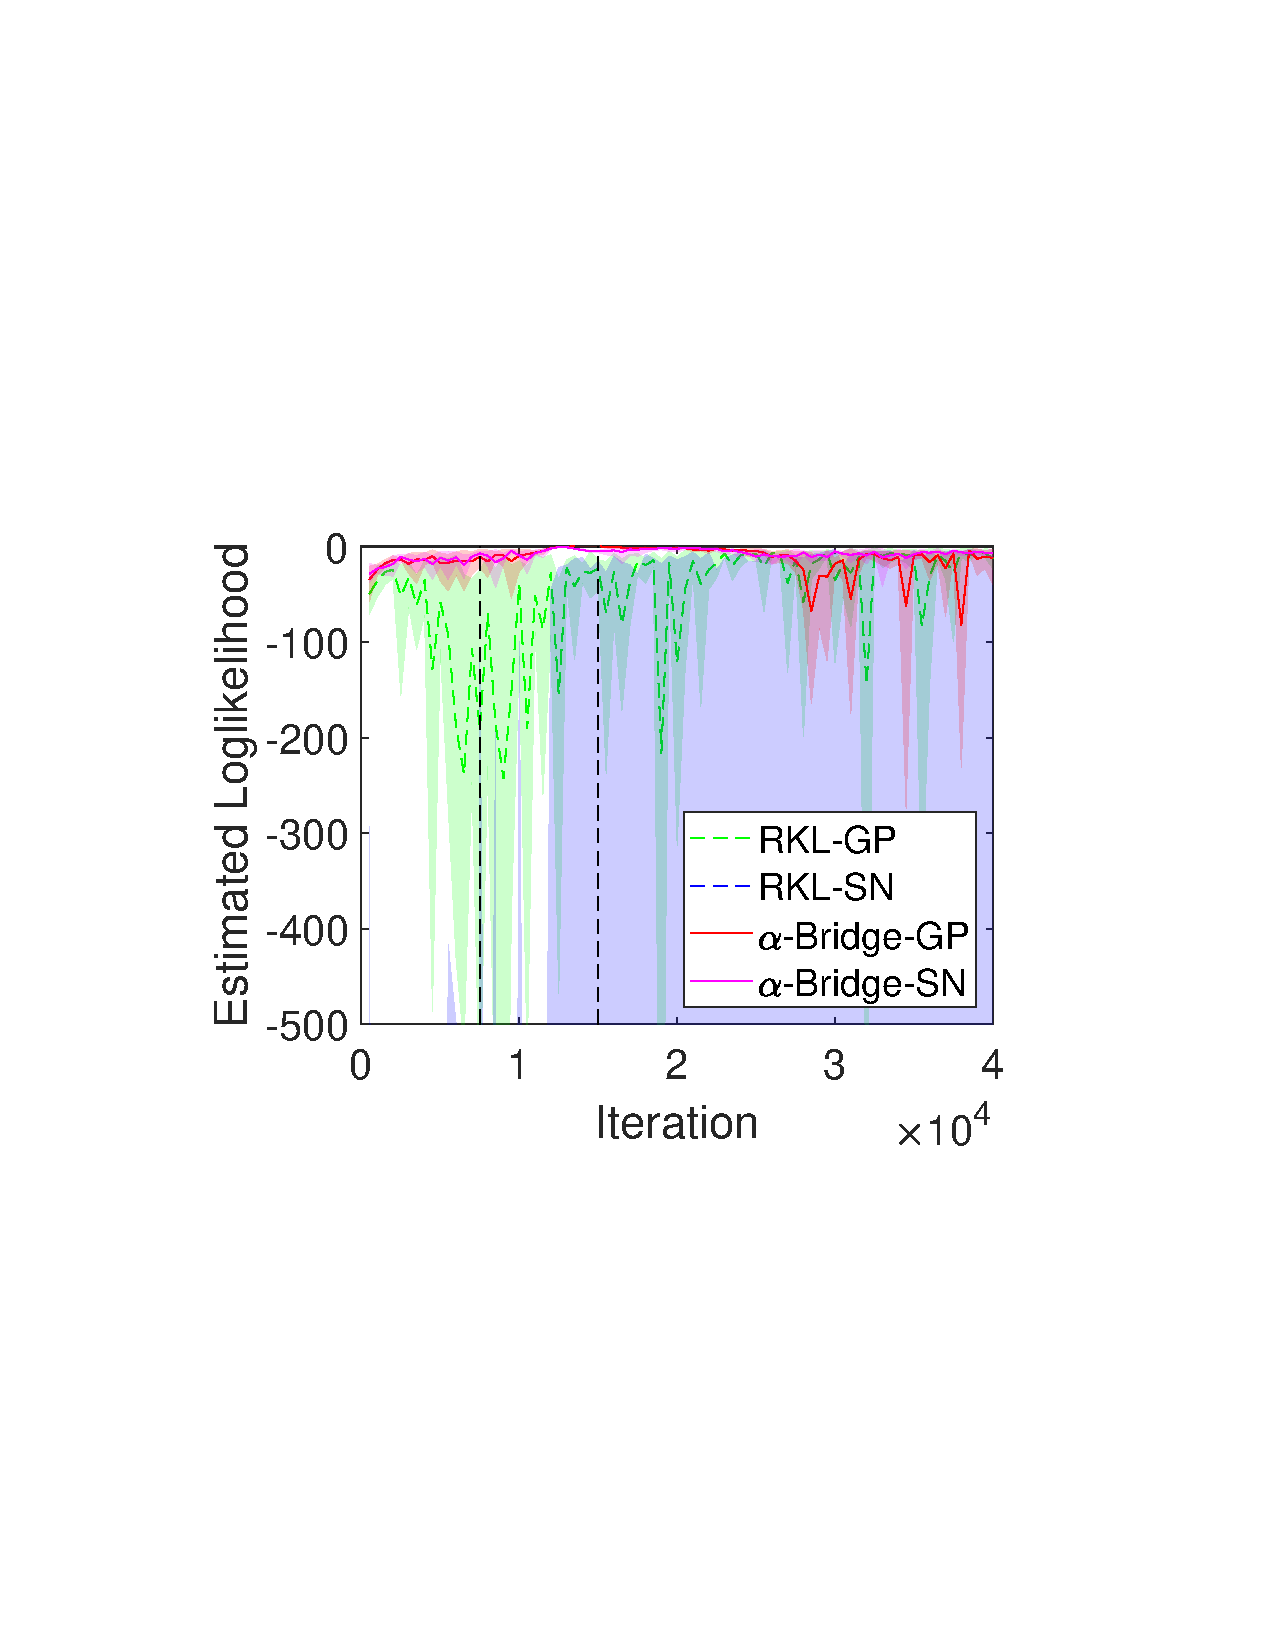
\includegraphics[height=0.33 \columnwidth]{Figures/0-5KL_25Gs_4comErr_loglikehood_2e4_0_5.pdf}
	}
	\caption{Quantitative performance of the methods along the training process.
		Inception score (a)$/$(c) and estimated log-likelihood (b)$/$(d) when Adam \cite{kingma2014adam} hyperparameter $\beta_1=0.1$ $/$ $\beta_1=0.5$.
		Higher is better for both metrics.
		The curves are calculated over $10$ random trials.
		Two vertical dashed lines are used to indicate the three steps of the $\alpha$-Bridge.
	}
	\label{fig:25Gs_IS_LL}
\end{figure}


We demonstrate the proposed $\alpha$-Bridge from three perspectives.
First we show that the $\alpha$-Bridge, dynamically transferring advantages from ML to adversarial learning, exhibits a more stable training with improved robustness to hyperparameters (this is expected because of the aforementioned discussions of control variants interpretation and connections to prior GAN regularization methods).
We then show that the $\alpha$-Bridge is capable of smoothly transferring the information learned during ML learning to adversarial learning, circumventing the forgetting issue shown in Figure \ref{fig:explodes}.
Finally we highlight the versatility of the $\alpha$-Bridge, by showing its capability in transplanting the variational approximation within ML learning into an inference arm for adversarial learning. See
%Appendix G
Appendix \ref{sec:app_exp}
for the detailed experimental settings.


\subsection{Stability and Robustness}
\label{sec:exp_25Gaussian}


The $25$-Gaussians example from \cite{tao2018chi} is adopted, where the data are generated from a 2D Gaussian mixture model with $25$ components, as shown in Figure \ref{fig:Sample_25G}. For direct comparison, reverse-KL-based GANs are chosen as baselines, with recent techniques to stabilize their training, \ie gradient penalty (GP) \cite{mescheder2018training} and spectral normalization (SN) \cite{miyato2018spectral}. Note it is shown in \cite{GoogleCompareGAN} that most GANs with the same budgets can reach similar performance with enough hyperparameter optimization and random restarts. Thus reverse-KL-based GANs further stabilized by GP/SN are considered as fairly good baselines (named as RKL-GP and RKL-SN, respectively)\footnote{Empirically, RKL-GP and RKL-SN show comparable/better results than WGAN-GP \cite{gulrajani2017improved} on $25$-Gaussians.}.
The inception score (IS) \cite{salimans2016improved} and the log-likelihood estimated with kernel density estimation \cite{parzen1962estimation} are used to measure the plausibility of generated samples and the data-mode-covering level of learned models, respectively.
Baseline methods are carefully tuned with their best settings adopted for fair comparison (see
%Appendix G.2).
Appendix \ref{sec:app_tuningbase_25Gs}).

Figure \ref{fig:25Gs_IS_LL} shows the results of the considered methods.
It is clear that $\alpha$-Bridge, thanks to its smooth transferring nature, is capable of benefiting from the advantages of ML learning, resulting in more stable training (see Figures \ref{fig:25Gs_4IS_0_1} and \ref{fig:25Gs_4IS_0_5}) while keeping most data modes covered (see Figures \ref{fig:25Gs_4LL_0_1} and \ref{fig:25Gs_4LL_0_5}).
Comparing Figures \ref{fig:25Gs_4IS_0_1}-\ref{fig:25Gs_4LL_0_1} to Figures \ref{fig:25Gs_4IS_0_5}-\ref{fig:25Gs_4LL_0_5} shows $\alpha$-Bridge is relatively more robust to hyperparameters than baseline methods (see
%Appendix G.2
Appendix \ref{sec:app_tuningbase_25Gs}
for more details).
Figure \ref{fig:Sample_25G} shows one training curve of the compared methods, highlighting $\alpha$-Bridge's ability to benefit from the advantages of ML learning.
To address the concern of how $\alpha$-Bridge performs on real datasets, we conduct another experiment on CIFAR$10$ \cite{krizhevsky2009learning}
and observe an improved performance of (IS, FID\cite{heusel2017gans})=$(7.225, 28.083)$ over $(6.558, 33.707)$ of the vanilla DCGAN baseline (see
%Appendix G.4
Appendix \ref{sec:app_exp_cifar10}
for more results).


\subsection{Smooth Transfer of Information from ML to Adversarial Learning}
%\label{sec:}

Besides inheriting the advantages of ML learning, another advantage of the $\alpha$-Bridge is a smooth transfer of the information learned during ML to adversarial learning.
For an explicit demonstration, we run $\alpha$-Bridge on the MNIST \cite{lecun1998gradient} and CelebA \cite{liu2015deep} datasets, and present the generated samples along the training process, as shown in Figure \ref{fig:Sample_MNIST_CelebA}.
ML learning, \ie Step $I$ of Algorithm \ref{alg:Alpha-divergence}, provides fairly good initialization on both datasets; thanks to the zero-avoiding nature of ML learning, one might anticipate an initialization covering all data modes, similar to the phenomena observed in Figure \ref{fig:Sample_25G}.
When it comes to the transferring Step $I\!I$, $\alpha$-Bridge smoothly inherits what's learned in ML learning at the beginning, and then gradually adds more detailed information (such as sharper edges on MNIST digits and clearer background on CelebA faces) to generate increasingly realistic images.
After the transferring Step $I\!I$, one observes generated images exhibiting the features from adversarial learning, whose image quality is further refined by the adversarial Step $I\!I\!I$ of Algorithm \ref{alg:Alpha-divergence}.
By reviewing the whole process shown in Figure \ref{fig:Sample_MNIST_CelebA}, one observes that $\alpha$-Bridge is capable of smoothly transferring most information from ML to adversarial learning, in contrast to the forgetting shown in Figure \ref{fig:explodes}.



\begin{figure}[tb]
	\centering
%		\includegraphics[height=0.33\columnwidth]{MNIST_alpha_bridge.pdf}
%		\includegraphics[height=0.60\columnwidth]{sample_celebA_5x10.pdf}
		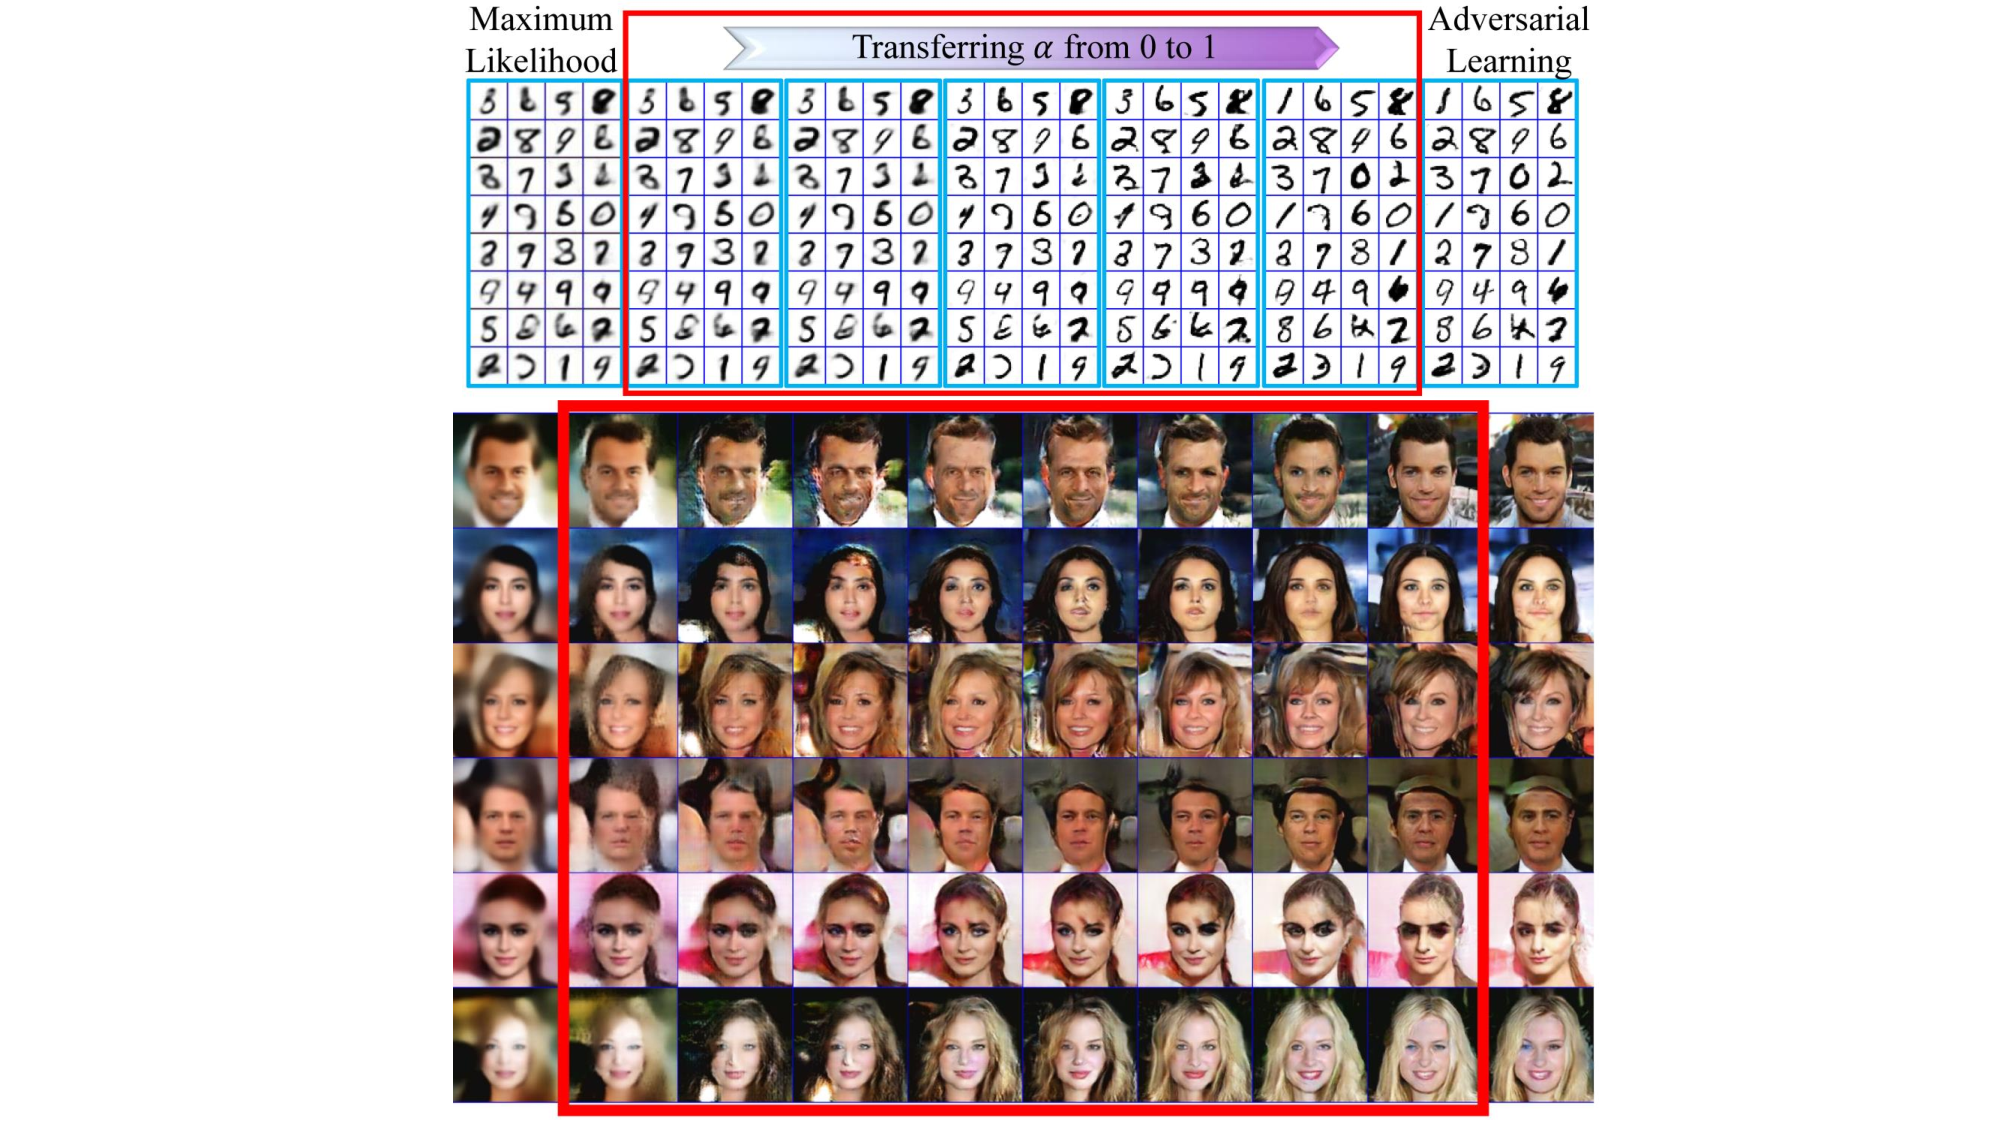
\includegraphics[width=\columnwidth]{Figures/MNIST_CelebA_transfer.pdf}
		\caption{Random samples generated along the training process of the $\alpha$-bridge on MNIST (top) and CelebA (bottom).
			Note most information is transferred from ML to adversarial learning, such as the class, rotation, and style of generated digits, and the basic tone, gender, expression, pose of the head, hair style of generated faces.
		}
		\label{fig:Sample_MNIST_CelebA}
\end{figure}



\subsection{Transplanting ML Variational Posterior into Inference Arm for Adversarial Learning}
%\label{sec:}



\begin{figure}[tb]
	\centering
%		\includegraphics[height=0.33 \columnwidth]{fake_recon_CELEB.pdf}
%		\includegraphics[height=0.55 \columnwidth]{Attribute_infer_arm_new.pdf}
		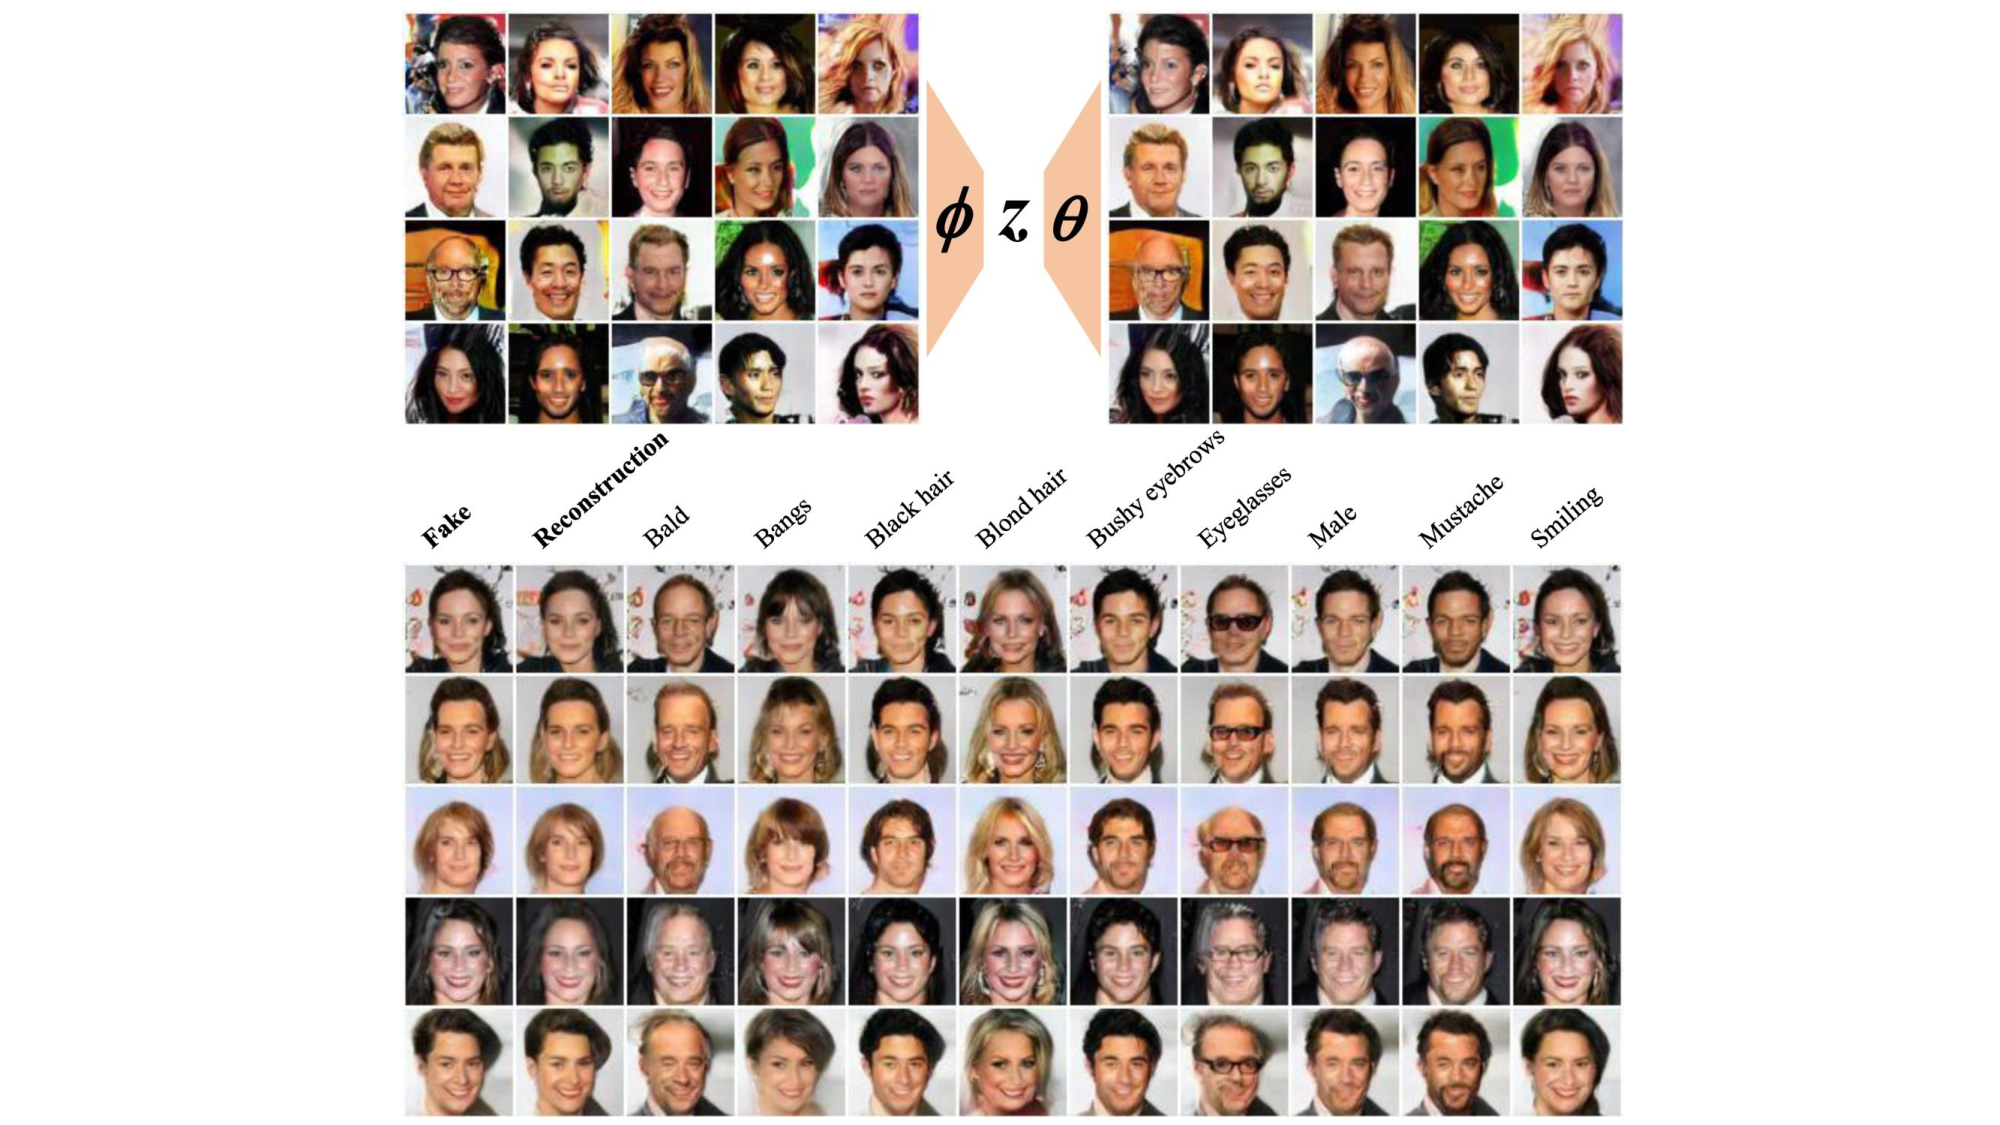
\includegraphics[width= \columnwidth]{Figures/Recon_Attribute_infer_CelebA.pdf}
		\caption{Using the inference arm transplanted by $\alpha$-Bridge to reconstruct (top) and manipulate (bottom) GAN generated images.
			$\phiv$ and $\thetav$ denote the inference arm $q_{\phiv}(\zv|\xv)$ and the generator $G_{\thetav}(\zv)$, respectively.
		}
		\label{fig:attribute_inference_arm}
\end{figure}

In addition to inheriting the advantages and information from ML learning, we find that the smooth dynamical training of Algorithm \ref{alg:Alpha-divergence} also enables $\alpha$-Bridge to transplant the variational approximation within ML learning into an inference arm for adversarial learning. Such a capacity is  appealing because it enables exploiting the generative power of GANs for various practical applications.
See
%Appendix G.6
Appendix \ref{sec:app_TransInferArm}
for technical details.


To verify the effectiveness of the transplanted inference arm, Figure \ref{fig:attribute_inference_arm} (top) shows the encoder-decoder reconstruction for the generated fake images. It is apparent that the reconstructions are fairly good, confirming the effectiveness of the inference arm.
One can also exploit that arm for manipulation of GAN generated images, as shown in Figure \ref{fig:attribute_inference_arm} (bottom). Detailed implementations for reconstruction and manipulation are given in
%Appendix G.6.
Appendix \ref{sec:app_TransInferArm}.
It is clear that with this inference arm, one can modify the semantic concepts of the generated images like bangs, hair, gender, \etc Such capacity is valuable for transferring the generative power of GANs to various down-steaming tasks.



\section{Conclusions}


Motivated by the fact that maximum likelihood (ML) and adversarial learning have complementary characteristics, we have proposed a novel $\alpha$-Bridge, constituted via the $\alpha$-divergence, to unify their advantages in a principled manner.
Our $\alpha$-Bridge has as its foundation newly recognized twin gradients of the $\alpha$-divergence, one of which utilizes the gradient information from the ML (forward KL) perspective, and the other from the adversarial learning (reverse KL) perspective.
We also have revealed two generalizations of $\alpha$-Bridge
that closely resemble CycleGAN \cite{zhu2017unpaired} and ALICE \cite{li2017alice}.


\subsubsection{Acknowledgments.} The research was supported by part by DARPA, DOE, NIH, NSF and ONR. The Titan Xp GPU used was donated by the NVIDIA Corporation.


\fontsize{9.0pt}{10.0pt}\selectfont
%\small
Magnam hic sed labore neque, vel facere laboriosam at hic placeat nihil possimus doloremque repudiandae tempora voluptatibus, corporis neque molestias atque porro excepturi voluptas, rerum minus quidem sequi eum nisi nobis enim explicabo asperiores, autem totam exercitationem culpa et sed?Ducimus labore voluptatum tenetur, inventore reprehenderit quo eos vitae laudantium maxime veniam minus error.Nobis tempora labore necessitatibus est mollitia quos sint deleniti a ducimus accusamus, sit dolore explicabo, optio nobis modi sunt error iste dolorum totam minus sequi possimus praesentium?Id autem assumenda ducimus exercitationem vitae accusamus quod, repudiandae voluptate enim totam aliquid officiis eum reprehenderit inventore nemo, maiores exercitationem tempora?Odio amet consequuntur sint animi, voluptatum rerum earum laboriosam.Dolor nobis ut veritatis optio odit saepe at, quos explicabo vero minus illo iste fugit aperiam, provident voluptates quos natus doloribus expedita suscipit, fugiat ipsum iure quod fuga illo neque eos tempore et, doloribus vero ipsam veniam a earum rem iure voluptatibus optio?Deleniti voluptate nam, corrupti natus aliquam est rerum ipsum tempora in laborum fugiat illo, itaque maiores atque maxime unde explicabo aliquam laboriosam nemo, consectetur culpa ad minus nulla corporis tenetur?Delectus optio voluptatem nulla reprehenderit atque, sunt reiciendis excepturi.Eius necessitatibus illum eum atque aut, totam impedit deserunt eligendi, nulla temporibus ipsam quae incidunt corporis laborum illum asperiores cumque, ea obcaecati reprehenderit perspiciatis nisi est labore voluptate hic odio inventore quisquam, corrupti corporis possimus vel ab placeat itaque sit assumenda.Voluptas totam unde omnis ipsum est quod mollitia sit ipsa qui adipisci, hic perspiciatis adipisci ex ullam, sunt facilis dolorem facere perferendis est voluptatem dignissimos sint obcaecati optio, doloremque accusantium quo ab, reprehenderit recusandae qui asperiores porro natus.Corporis et quia fugiat, repellat illo ducimus harum accusantium culpa doloribus architecto pariatur alias eius neque?Vero provident nostrum fugit omnis, itaque ad autem voluptatem ipsum aspernatur ex quia repudiandae quos, ut laudantium officiis quae mollitia accusamus magni deserunt nesciunt?Quam nulla beatae temporibus perspiciatis neque repellendus perferendis optio, modi similique voluptas architecto alias ab incidunt expedita quaerat atque, cupiditate quaerat tenetur temporibus provident consequuntur unde totam dignissimos, placeat obcaecati vero eos earum tenetur hic?\clearpage
\bibliography{ReferencesCong}
\bibliographystyle{aaai}


\normalsize

\end{document}

